%!TEX TS-program = xelatex
\documentclass[notes,12pt, aspectratio=169]{beamer}

\usepackage{amsmath,amsfonts,amssymb,amsthm,mathtools}  % пакеты для математики
\usepackage{minted}

\usepackage[english, russian]{babel} % выбор языка для документа
\usepackage[utf8]{inputenc} % задание utf8 кодировки исходного tex файла
\usepackage[X2,T2A]{fontenc}        % кодировка

\usepackage{fontspec}         % пакет для подгрузки шрифтов
\setmainfont{Helvetica}  % задаёт основной шрифт документа

% why do we need \newfontfamily:
% http://tex.stackexchange.com/questions/91507/
\newfontfamily{\cyrillicfonttt}{Helvetica}
\newfontfamily{\cyrillicfont}{Helvetica}
\newfontfamily{\cyrillicfontsf}{Helvetica}

\usepackage{unicode-math}     % пакет для установки математического шрифта
% \setmathfont{Neo Euler} % шрифт для математики

\usepackage{polyglossia}      % Пакет, который позволяет подгружать русские буквы
\setdefaultlanguage{russian}  % Основной язык документа
\setotherlanguage{english}    % Второстепенный язык документа

% Шрифт для кода
\setmonofont[Scale=0.85]{Monaco}
\usepackage{verbments}

\usepackage{pgfpages}
% These slides also contain speaker notes. You can print just the slides,
% just the notes, or both, depending on the setting below. Comment out the want
% you want.
%\setbeameroption{hide notes} % Only slide
%\setbeameroption{show only notes} % Only notes
%\setbeameroption{show notes on second screen=right} % Both

\usepackage{array}

\usepackage{tikz}
\usepackage{verbatim}
\setbeamertemplate{note page}{\pagecolor{yellow!5}\insertnote}
\usetikzlibrary{positioning}
\usetikzlibrary{snakes}
\usetikzlibrary{calc}
\usetikzlibrary{arrows}
\usetikzlibrary{decorations.markings}
\usetikzlibrary{shapes.misc}
\usetikzlibrary{matrix,shapes,arrows,fit,tikzmark}

\usepackage{hyperref}
\usepackage{lipsum}
\usepackage{multimedia}
\usepackage{multirow}
\usepackage{dcolumn}
\usepackage{bbm}
\newcolumntype{d}[0]{D{.}{.}{5}}

\usepackage{changepage}
\usepackage{appendixnumberbeamer}
\newcommand{\beginbackup}{
   \newcounter{framenumbervorappendix}
   \setcounter{framenumbervorappendix}{\value{framenumber}}
   \setbeamertemplate{footline}
   {
     \leavevmode%
     \hline
     box{%
       \begin{beamercolorbox}[wd=\paperwidth,ht=2.25ex,dp=1ex,right]{footlinecolor}%
%         \insertframenumber  \hspace*{2ex} 
       \end{beamercolorbox}}%
     \vskip0pt%
   }
 }
\newcommand{\backupend}{
   \addtocounter{framenumbervorappendix}{-\value{framenumber}}
   \addtocounter{framenumber}{\value{framenumbervorappendix}} 
}

% для имитации питоновского синтаксиса 
\newcommand{\pgr}[1]{{\color{green} \textbf{#1}}}


%%%%%%%%%% Работа с картинками %%%%%%%%%
\usepackage{graphicx}                  % Для вставки рисунков
\usepackage{graphics}
\graphicspath{{images_1/}}    % можно указать папки с картинками
\usepackage{wrapfig}                   % Обтекание рисунков и таблиц текстом

\usepackage[space]{grffile}
\usepackage{booktabs}

% These are my colors -- there are many like them, but these ones are mine.
\definecolor{blue}{RGB}{0,114,178}
\definecolor{red}{RGB}{213,94,0}
\definecolor{yellow}{RGB}{240,228,66}
\definecolor{green}{RGB}{0,128, 0}

\hypersetup{
  colorlinks=false,
  linkbordercolor = {white},
  linkcolor = {blue}
}


%% I use a beige off white for my background
\definecolor{MyBackground}{RGB}{255,253,218}

%% Uncomment this if you want to change the background color to something else
%\setbeamercolor{background canvas}{bg=MyBackground}

%% Change the bg color to adjust your transition slide background color!
\newenvironment{transitionframe}{
  \setbeamercolor{background canvas}{bg=yellow}
  \begin{frame}}{
    \end{frame}
}

\setbeamercolor{frametitle}{fg=blue}
\setbeamercolor{title}{fg=black}
\setbeamertemplate{footline}[frame number]
\setbeamertemplate{navigation symbols}{} 
\setbeamertemplate{itemize items}{-}
\setbeamercolor{itemize item}{fg=blue}
\setbeamercolor{itemize subitem}{fg=blue}
\setbeamercolor{enumerate item}{fg=blue}
\setbeamercolor{enumerate subitem}{fg=blue}
\setbeamercolor{button}{bg=MyBackground,fg=blue,}


% If you like road maps, rather than having clutter at the top, have a roadmap show up at the end of each section 
% (and after your introduction)
% Uncomment this is if you want the roadmap!
% \AtBeginSection[]
% {
%    \begin{frame}
%        \frametitle{Roadmap of Talk}
%        \tableofcontents[currentsection]
%    \end{frame}
% }
\setbeamercolor{section in toc}{fg=blue}
\setbeamercolor{subsection in toc}{fg=red}
\setbeamersize{text margin left=1em,text margin right=1em} 

% списки, которые растягиваются на всю величину слайда 
\newenvironment{wideitemize}{\itemize\addtolength{\itemsep}{10pt}}{\enditemize}


\title[]{\textcolor{blue}{Практический анализ данных и машинное обучение: искусственные нейронные сети}}
\author{Ульянкин Филипп и Соловей Влад}
\date{\today}



\begin{document}

%%% TIKZ STUFF
\tikzset{   
        every picture/.style={remember picture,baseline},
        every node/.style={anchor=base,align=center,outer sep=1.5pt},
        every path/.style={thick},
        }
\newcommand\marktopleft[1]{%
    \tikz[overlay,remember picture] 
        \node (marker-#1-a) at (-.3em,.3em) {};%
}
\newcommand\markbottomright[2]{%
    \tikz[overlay,remember picture] 
        \node (marker-#1-b) at (0em,0em) {};%
}
\tikzstyle{every picture}+=[remember picture] 
\tikzstyle{mybox} =[draw=black, very thick, rectangle, inner sep=10pt, inner ysep=20pt]
\tikzstyle{fancytitle} =[draw=black,fill=red, text=white]
%%%% END TIKZ STUFF

% Title Slide
\begin{frame}
\maketitle
\centering Введение в Нейросети
\end{frame}


{
	\usebackgroundtemplate{ 
	\hspace{3cm}	
\includegraphics[height=\paperheight]{ya.jpg}}
\begin{frame}
\end{frame}
}


\begin{frame}{Структура курса}
\begin{wideitemize}
	
	\item Введение в нейросетки
	
	\item Как обучаются нейросетки, эвристики, используемые при обучении
	
	\item Свёрточные нейронные сети
	
	\item Сети прямого распространения в анализе текстов
	
	\item Рекурентные нейросетки 
	
	\item Обзор современных нейросетевых конструкций (GANы, автопереводы, нейробайесовский подход и тп)
\end{wideitemize} 
\end{frame}


\begin{frame}{Что почитать про нейронки}
\begin{center}
	
\includegraphics[width=.8\linewidth]{books.png}
\end{center}
\end{frame} 


\begin{frame}{Что посмотреть  про нейронки}
\begin{wideitemize} 
\item Если ничего не знаете про машинное обучение, смотрите вводный курс от Яндекса и МФТИ: {\color{blue} \url{https://www.coursera.org/specializations/machine-learning-data-analysis}}

\item Серия лекций техносферы: {\color{blue} \url{https://www.youtube.com/watch?v=Am82yvUSwRE}}

\item  Введение в нейронные сети от Andrew Ng: {\color{blue} \url{https://www.coursera.org/instructor/andrewng}}

\item  Advanced ML от Яндекса: {\color{blue} \url{https://www.coursera.org/specializations/aml}}

\end{wideitemize} 
\end{frame} 




\begin{frame}{Agenda}
\begin{wideitemize}

\item Немного истории

\item Напоминание о линейных моделях, переобучении, регуляризаторах и кросс-валидации

\item Всё, что вы хотели знать о градиентном спуске, но боялись спросить

\item От линейных моделей к нейросеткам

\item Нейросетки  — конструктор Lego 

\end{wideitemize} 
\end{frame}


\begin{transitionframe}
	\begin{center}
		\Huge История нейросеток
	\end{center}
\end{transitionframe}


% тут закоменчены слайды с каспаровым, шахматами  и alpha_go

%\begin{frame}
%\begin{center}
%	\resizebox{0.51\linewidth}{!}{
%		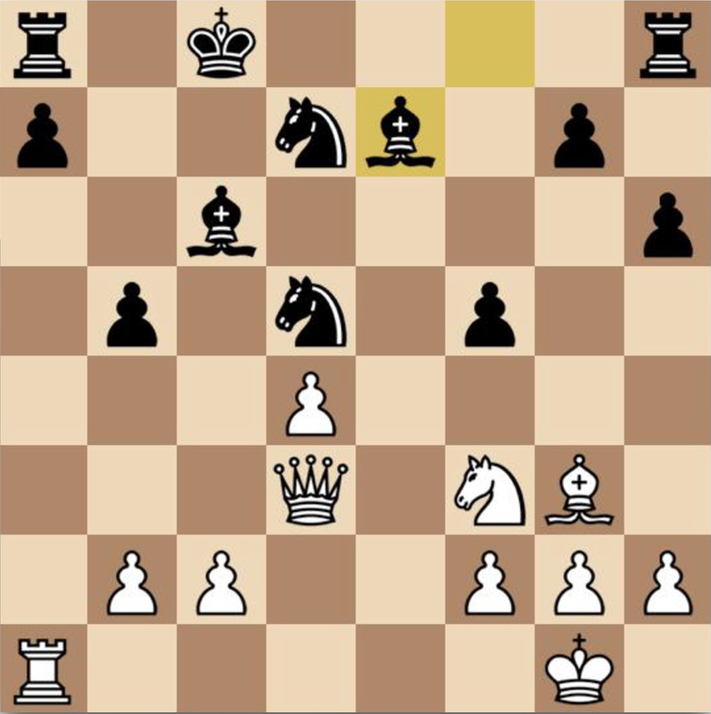
\includegraphics{chess_1.png}
%	}
%\end{center}
%\end{frame}


%\begin{frame}
%\begin{center}
%	\resizebox{0.51\linewidth}{!}{
%		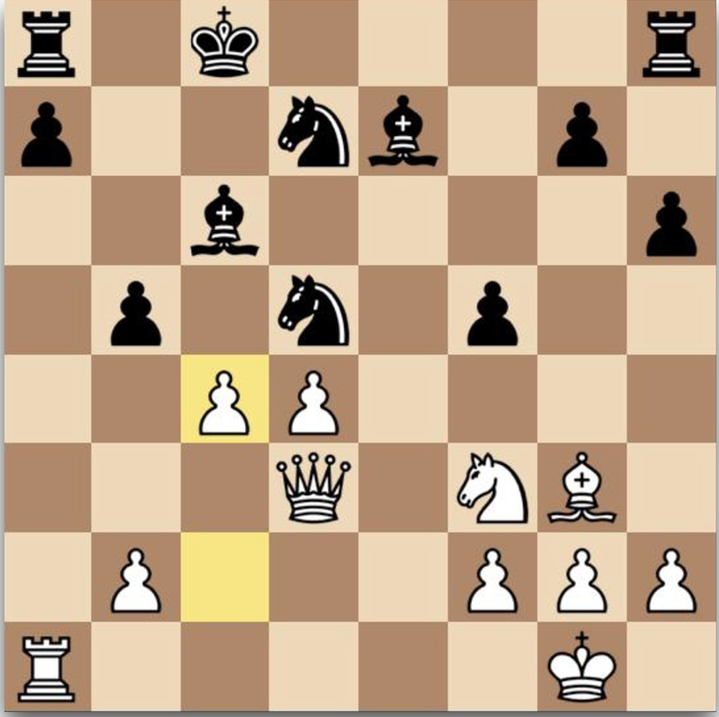
\includegraphics{chess_2.png}
%	}
%\end{center}
%\end{frame}


%\begin{frame}{ }
%\begin{columns}[T]
%\begin{column}{.49\textwidth}
%	\hspace{1.5cm}
%	\resizebox{0.51\linewidth}{!}{
%	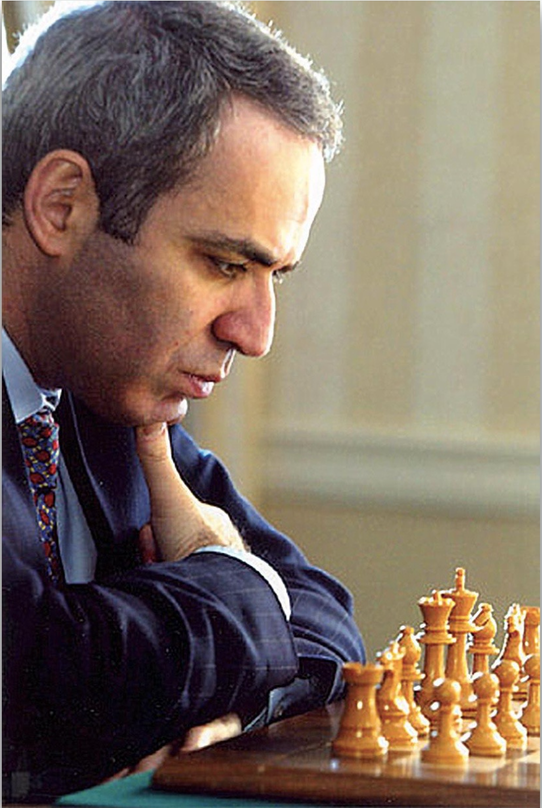
\includegraphics{kasparov.png}
%}
%\mbox{ }
%
%\hspace{1.9cm} Garry Kasparov
%\end{column}
%\hfill
%\begin{column}{.49\textwidth}
%%%% 
%\end{column}
%\end{columns}
%\end{frame}

%\begin{frame}
%\begin{columns}[T]
%	\begin{column}{.49\textwidth}
%		\hspace{1.5cm}
%		\resizebox{0.51\linewidth}{!}{
%			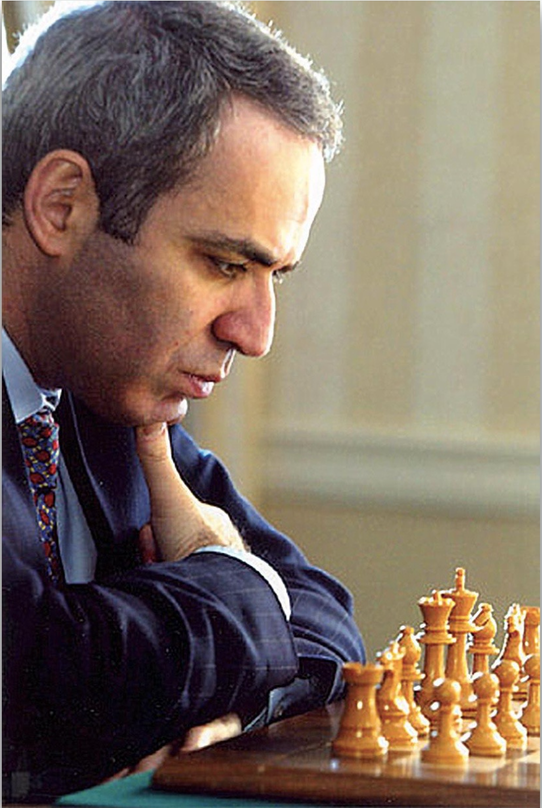
\includegraphics{kasparov.png}
%		}
%		\mbox{ }
%		
%		\hspace{1.9cm} Garry Kasparov
%	\end{column}
%	\hfill
%	\begin{column}{.49\textwidth}
%	\hspace{1.5cm}
%	\resizebox{0.51\linewidth}{!}{
%		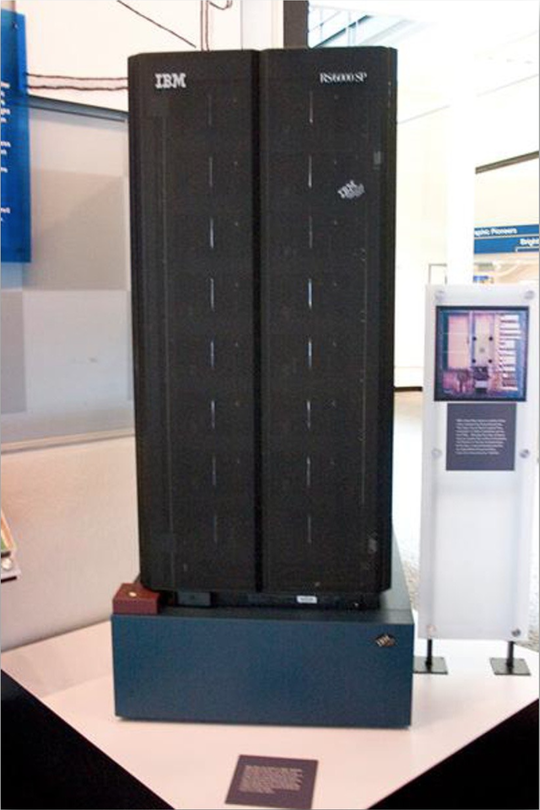
\includegraphics{deepblue.png}
%	}
%	\mbox{ }
%	
%	\hspace{2.5cm} Deepblue
%	\end{column}
%\end{columns}
%\end{frame}

%\begin{frame}
%\begin{center}
%	\resizebox{0.4\linewidth}{!}{
%		
\includegraphics{signal.jpg}
%	}
%\end{center}
%\end{frame}

%\begin{frame}
%\begin{wideitemize}
%	\item Шашки полностью решены в 2007 году 
%	\item Шахматы: впервые компьютер побеждает человека в феврале 1996 года 
%	\item Шахматы: в ноябре 2005 человек в последний раз побеждает у компьютера
%	\item Го: последний оплот человечества до апреля 2016 года
%\end{wideitemize} 
%\end{frame}

%\begin{frame}{GO пал со счётом 4 : 1}
%\begin{columns}[T]
%	\begin{column}{.49\textwidth}
%		\hspace{1.5cm}
%		\resizebox{0.51\linewidth}{!}{
%			
\includegraphics{alphago.png} 
%		} 
%		\mbox{ }
%		
%		\hspace{1.6cm} AlphaGo by Google
%	\end{column}
%	\hfill
%	\begin{column}{.49\textwidth}
%		\hspace{1.5cm}
%		\resizebox{0.51\linewidth}{!}{
%			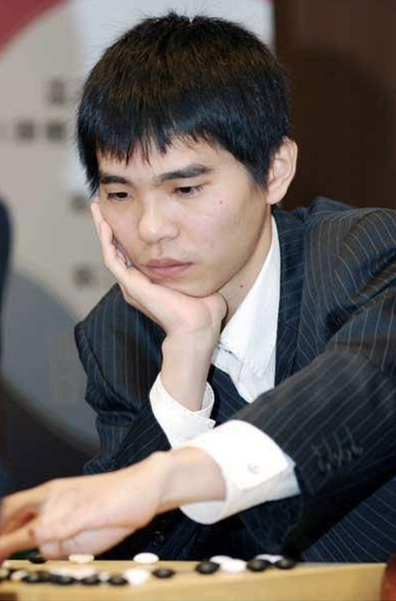
\includegraphics{lee_sedol.png}
%		}
%		\mbox{ }
%		
%		\hspace{2.5cm} Lee Sedol
%	\end{column}
%\end{columns}
%\end{frame}

%\begin{frame}
%\begin{center}
%	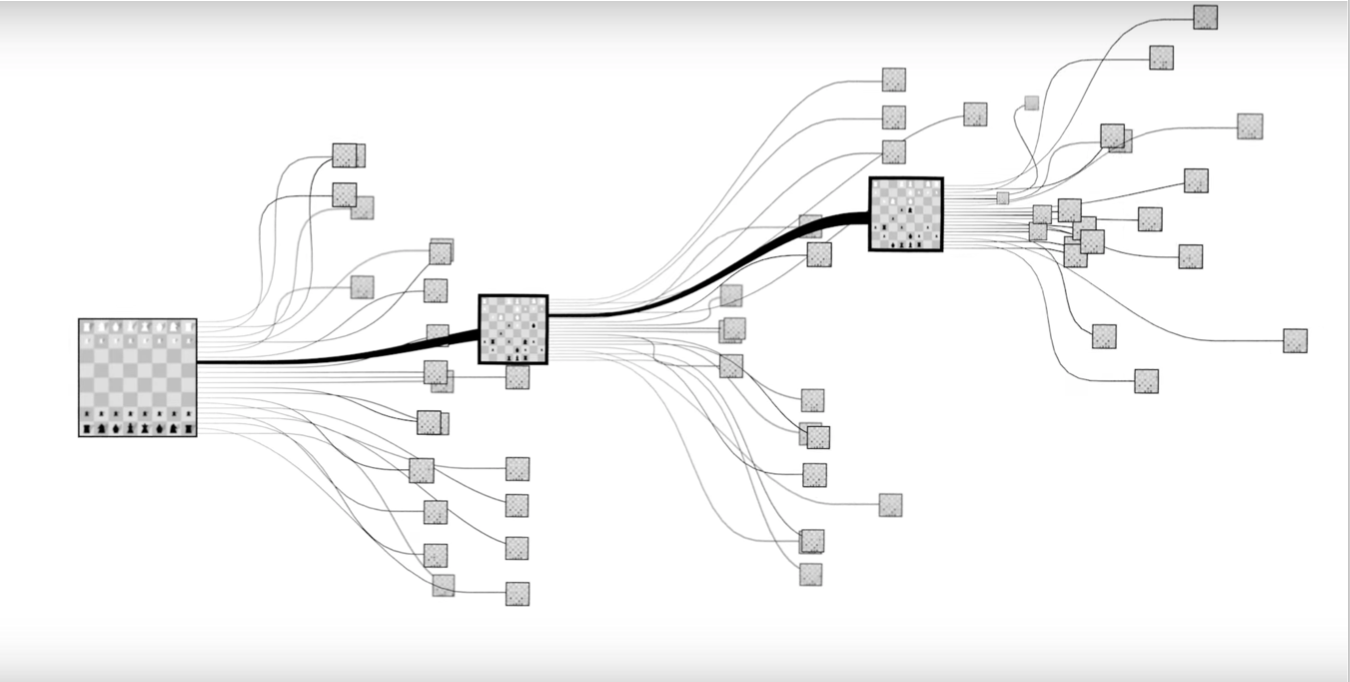
\includegraphics[width=.9\linewidth]{chees_3.png}
%\end{center}
%\end{frame}
%
%
%\begin{frame}
%\begin{center}
%	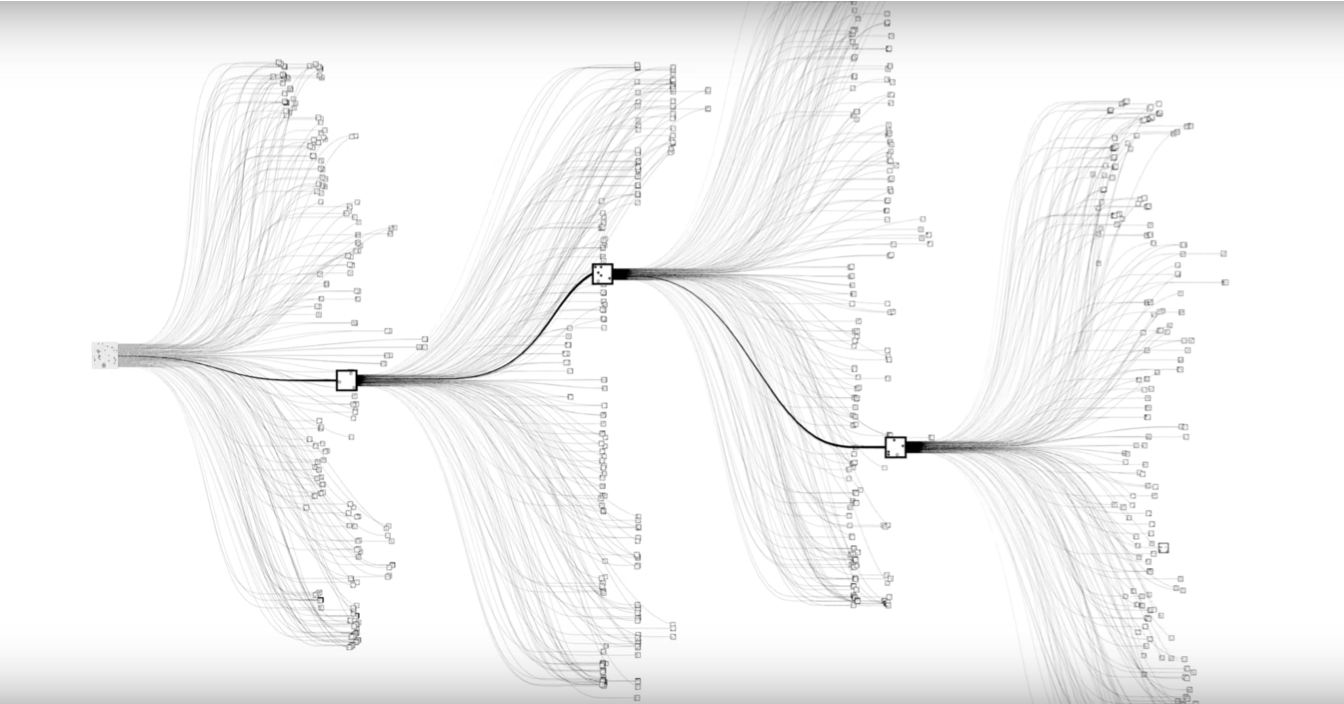
\includegraphics[width=.9\linewidth]{chess_4.png}
%\end{center}
%\end{frame}


% Отсюда начинаются слайды с нормальной историей 



\begin{frame}{Первый формальный нейрон, 1943 год}
\begin{center}
	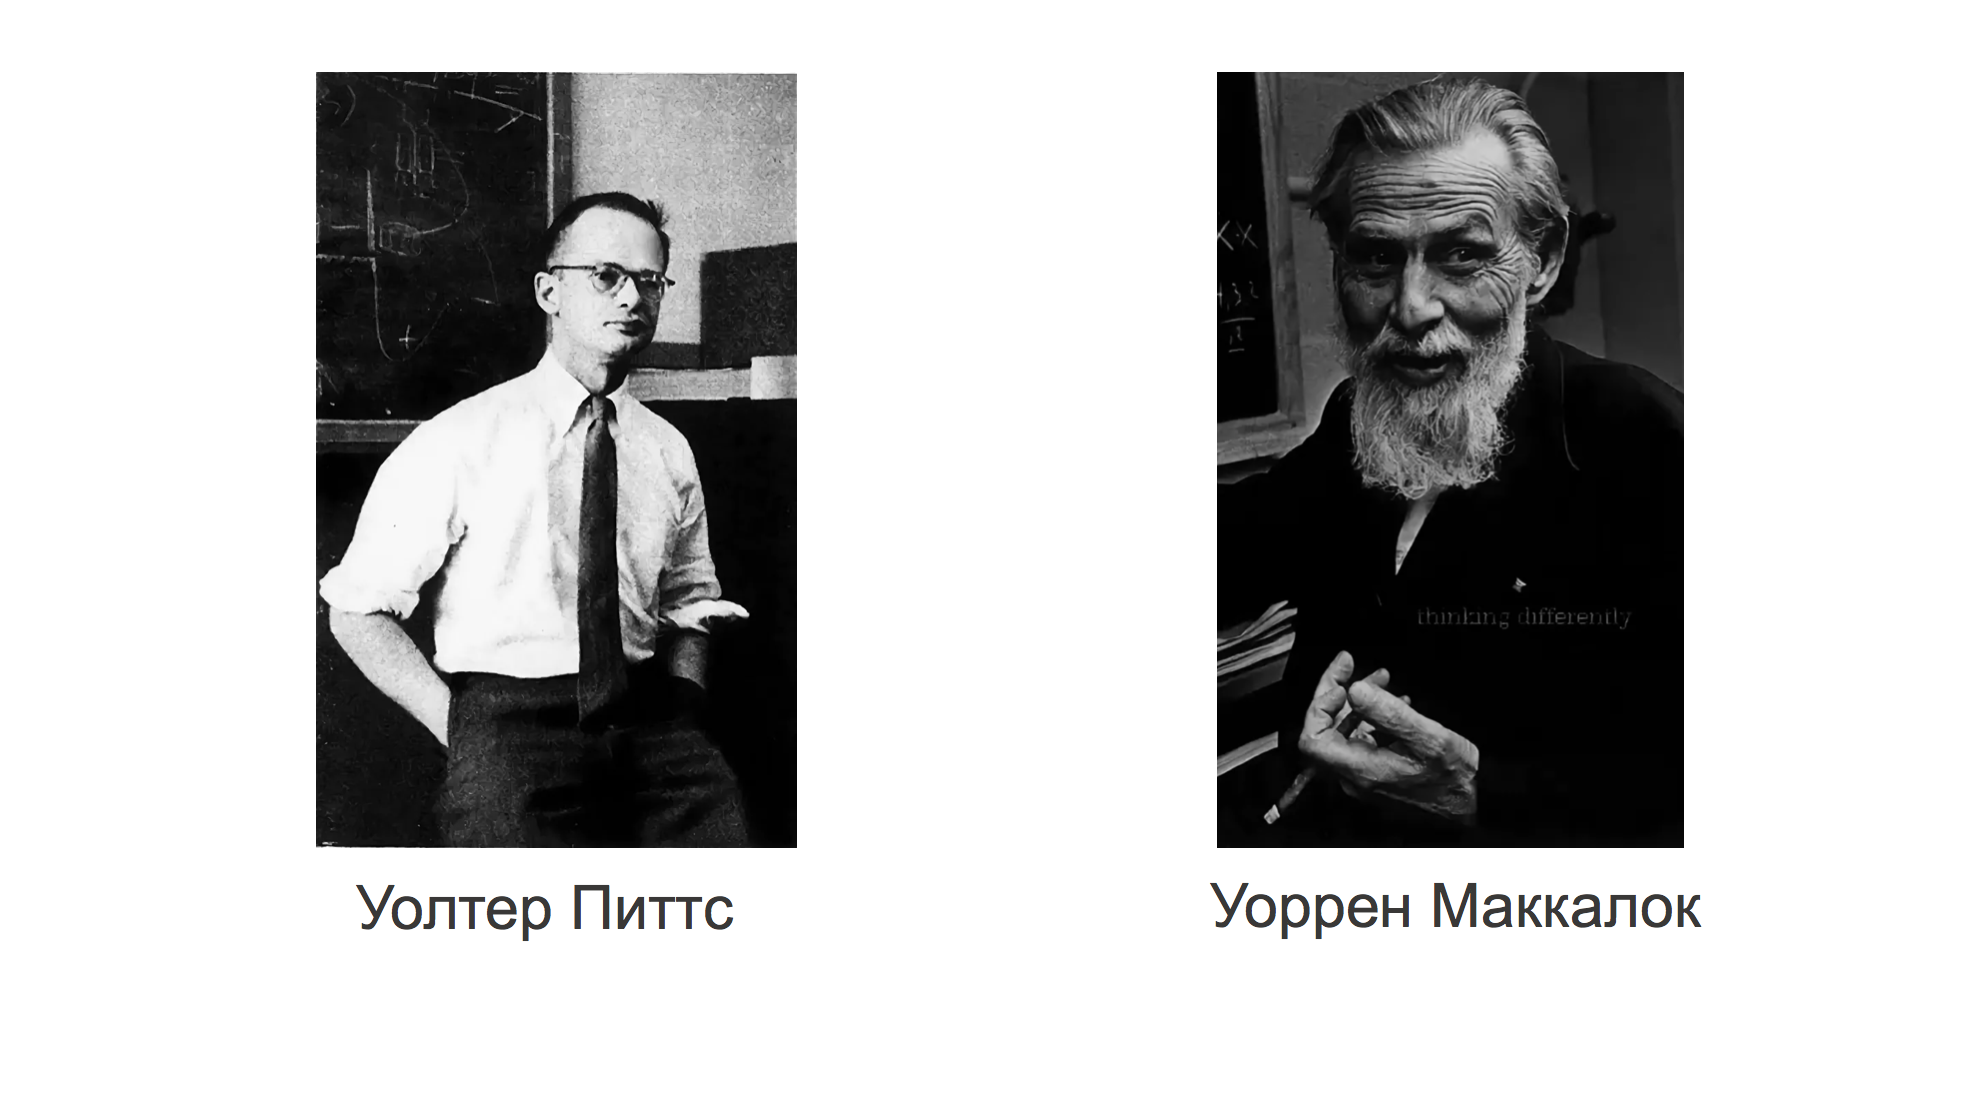
\includegraphics[width=0.9\paperwidth]{makkalok_pits.png}
\end{center}
\end{frame}


\begin{frame}{Первый искусственная нейросеть, 1958 год}
\begin{center}
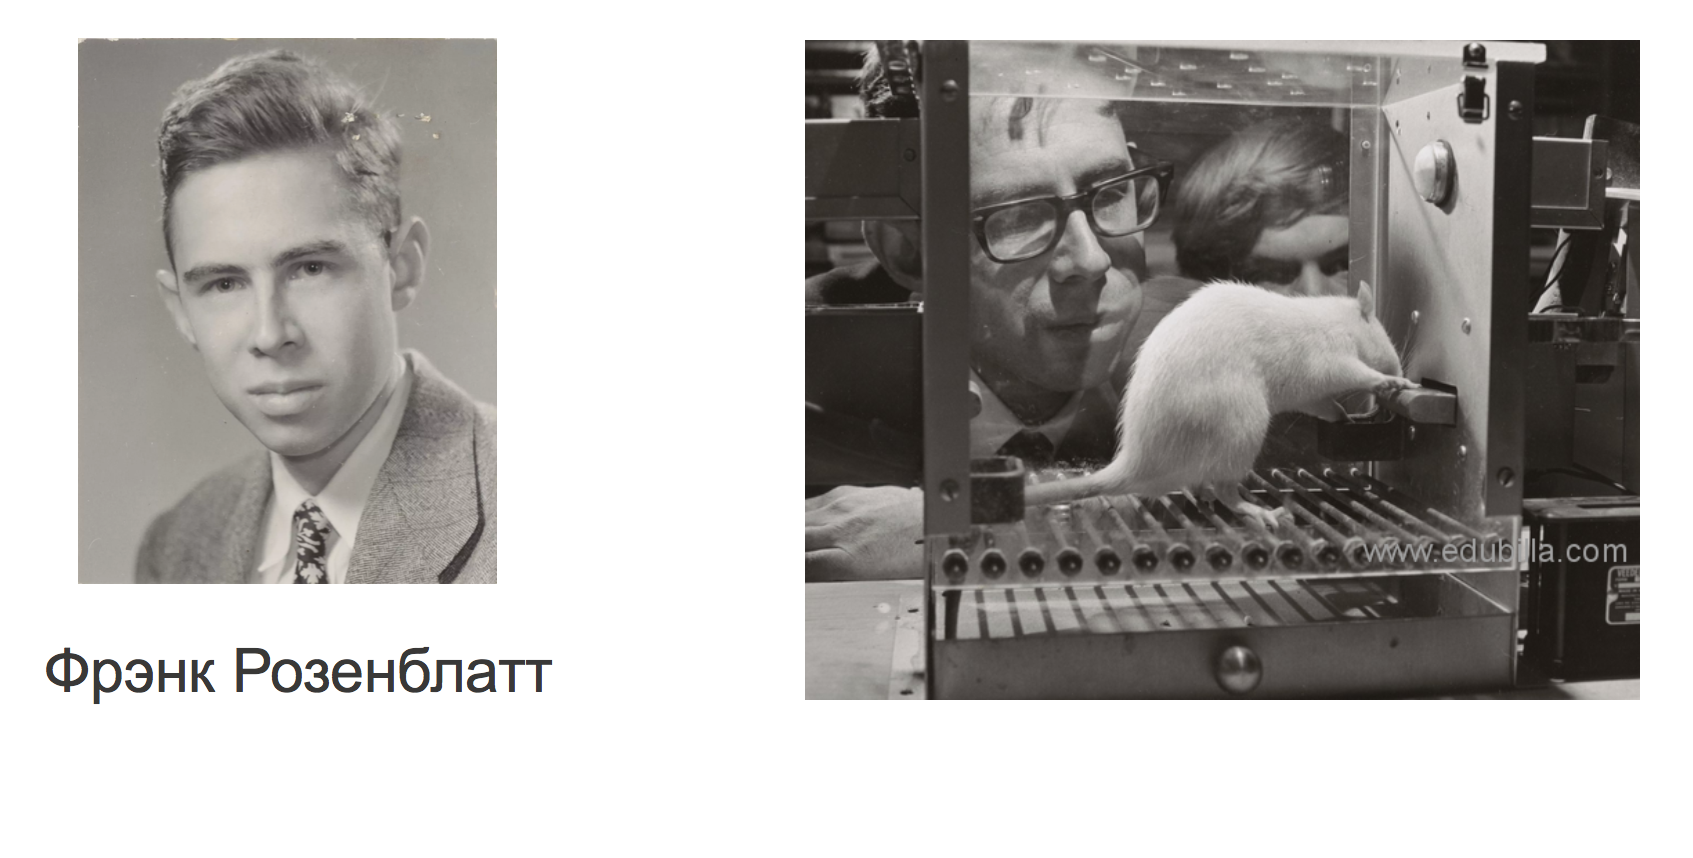
\includegraphics[width=0.9\paperwidth]{rozenblat.png}
\end{center}
\end{frame}


{
\usebackgroundtemplate{ 
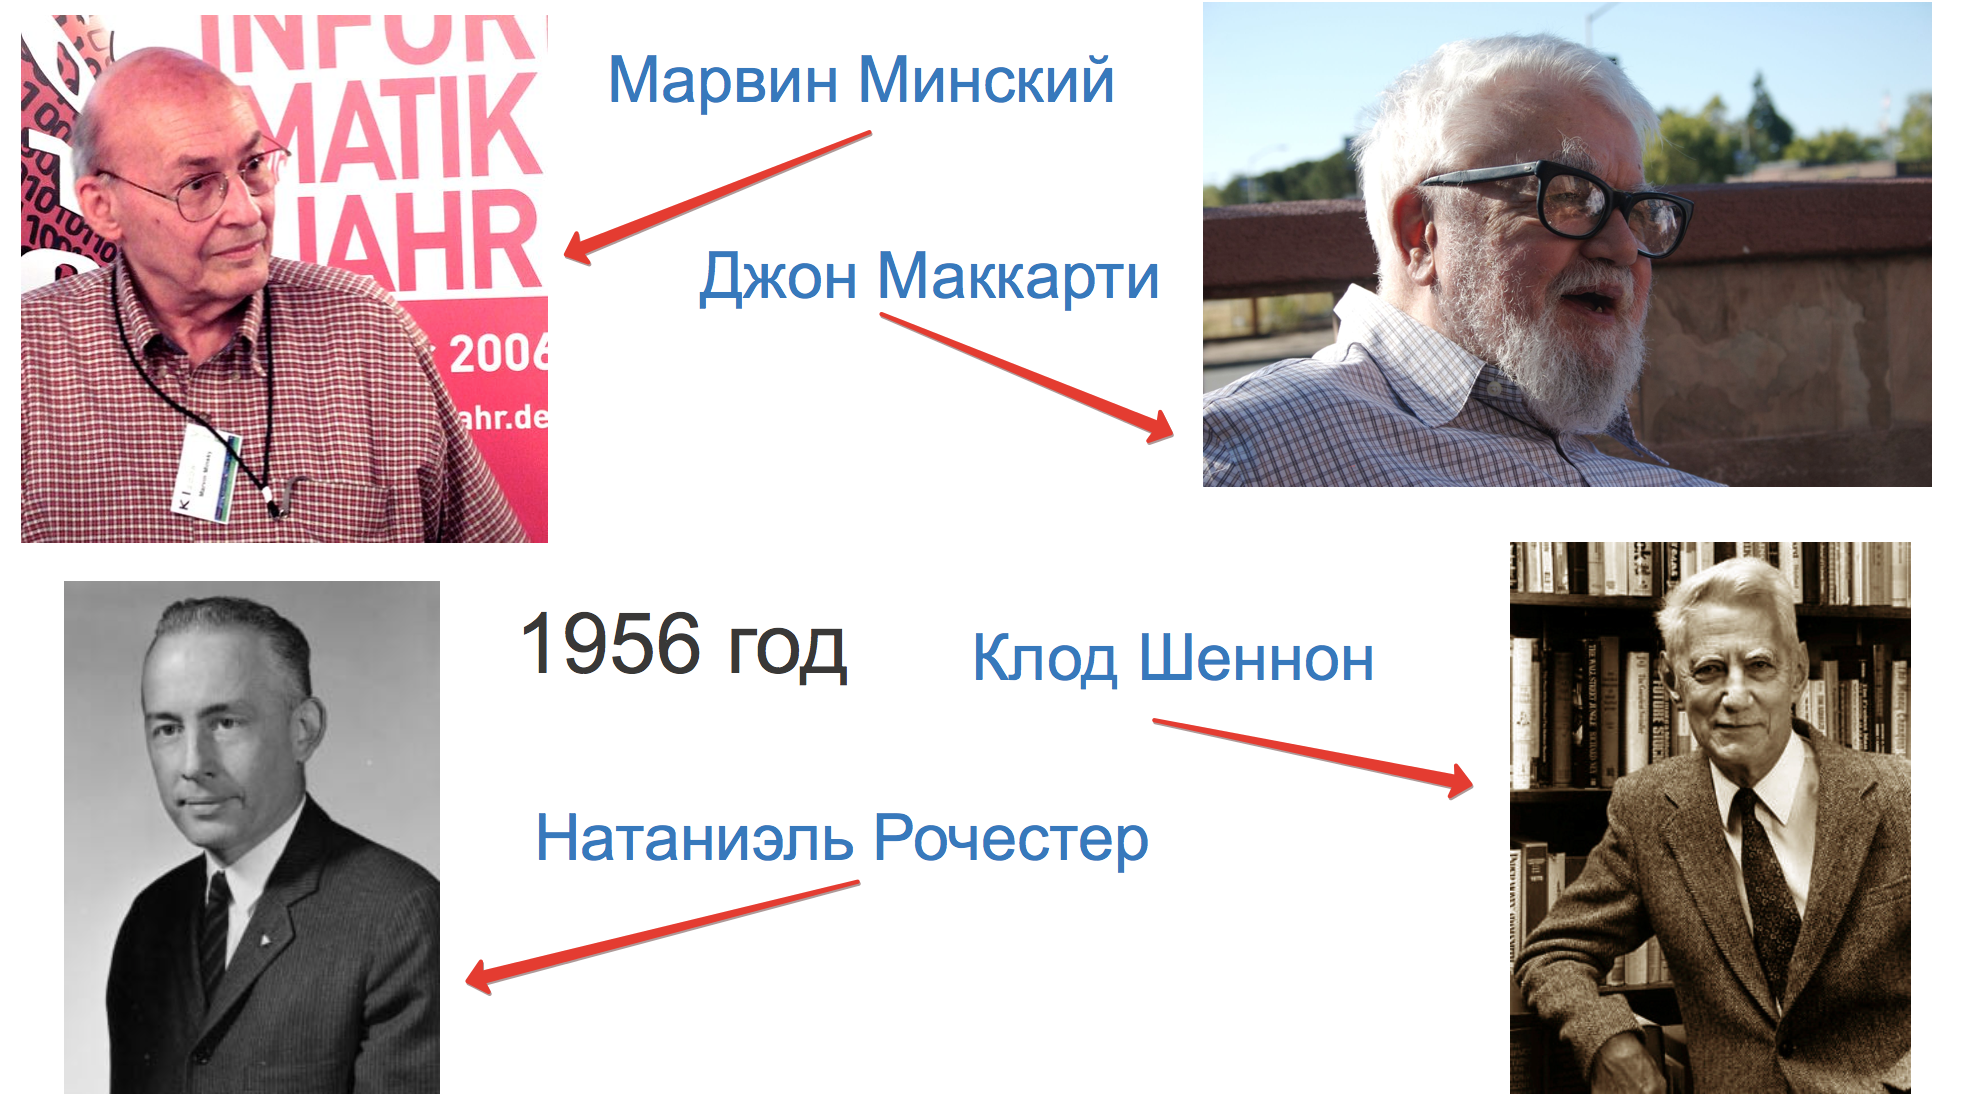
\includegraphics[width=\paperwidth]{dartmund_1.png}}
\begin{frame}
\end{frame}
}

{
\usebackgroundtemplate{ 
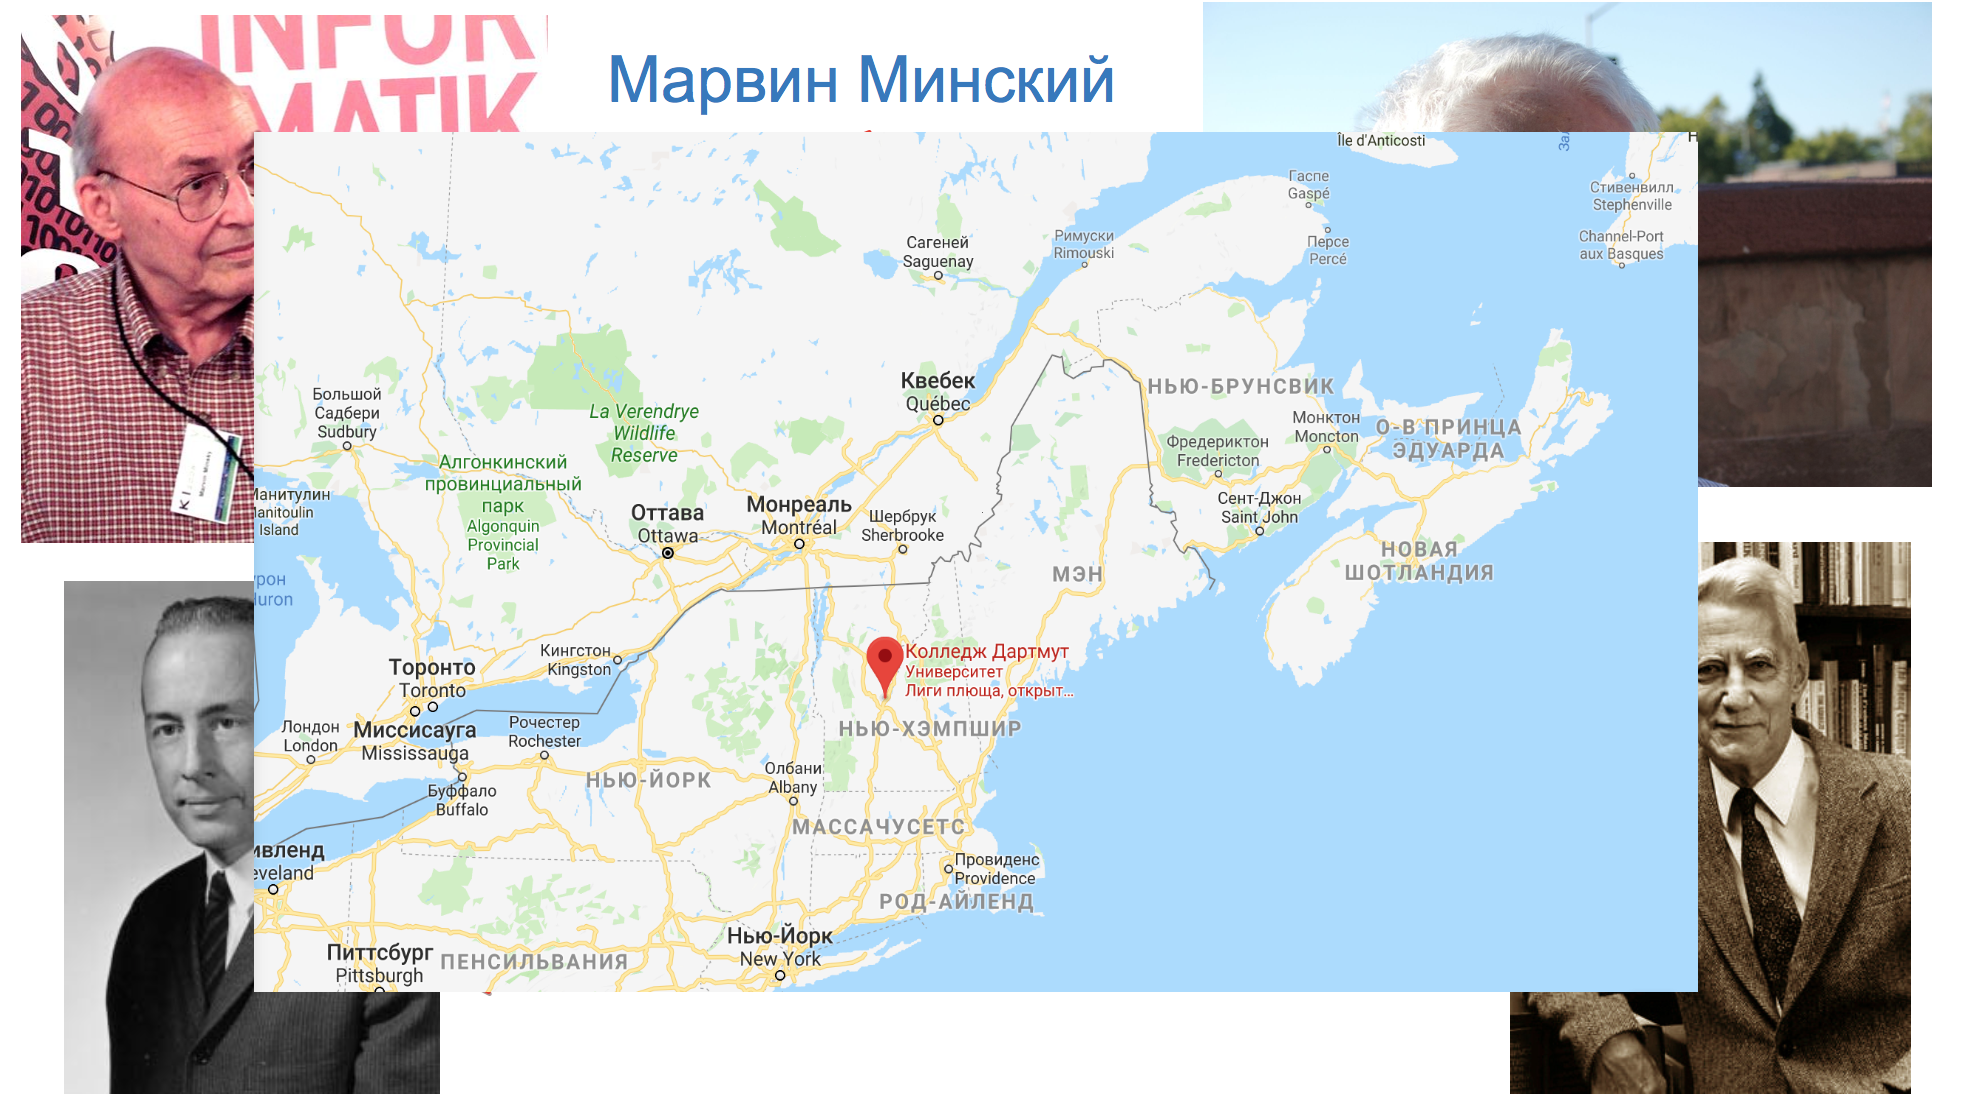
\includegraphics[width=\paperwidth]{dartmund_2.png}}
\begin{frame}
\end{frame}
}

\begin{frame}{Зима близко}
\begin{columns}[T] 
\begin{column}{.5\textwidth}
\begin{wideitemize} 
\item 1956 — Дартмунтский семинар, море оптимизма

\item 1958 — Перцептрон Розенблатта

\item середина 1960-х — провал крупного проекта по машинному переводу с русского на английский и наоборот 

\item 1969 — Марвин Минский и Сеймур Пейперт опубликовали книгу «Перцептроны» с критикой 

\end{wideitemize} 
\end{column}%
\hfill%
\begin{column}{.5\textwidth}
\begin{center}

\includegraphics[width=.99\linewidth]{stark.jpg}
\end{center}
\end{column}%
\end{columns}
\end{frame}



\begin{frame}{Оттепель}
\begin{wideitemize} 
\item 1970-е — Расцвет экспертных систем, принимающих решения на основе большого числа правил и знаний о предметной области 

\item MYCIN накопила около $600$ правил для идентификации вирусных бактерий и выдачи подходящего метода лечения (угадывала в $69\%$ случаев, лучше любого начинающего врача)

\item 1980-е  — появилось много разных архитектур

\item 1980-е — backpropagation позволил обучать сети за линейное время

\item Ренессанс нейронных сетей 
\end{wideitemize} 
\end{frame}


\begin{frame}{Зима близко}
\begin{columns}[T] 
\begin{column}{.5\textwidth}
\begin{wideitemize} 
\item Новая волна оптимизма

\item 1986 — один из первых AI-отделов экономил компании DEC около 10 миллионов долларов в год

\item Завышенные ожидания снова лопнули

\item 1990-е — ударными темпами развивается классическое машинное обучение
\end{wideitemize} 
\end{column}%
\hfill%
\begin{column}{.5\textwidth}
\begin{center}

\includegraphics[width=.79\linewidth]{stark_2.png}
\end{center}
\end{column}%
\end{columns}
\end{frame}


\begin{frame}{2005-2006: начало революции}
\begin{center}
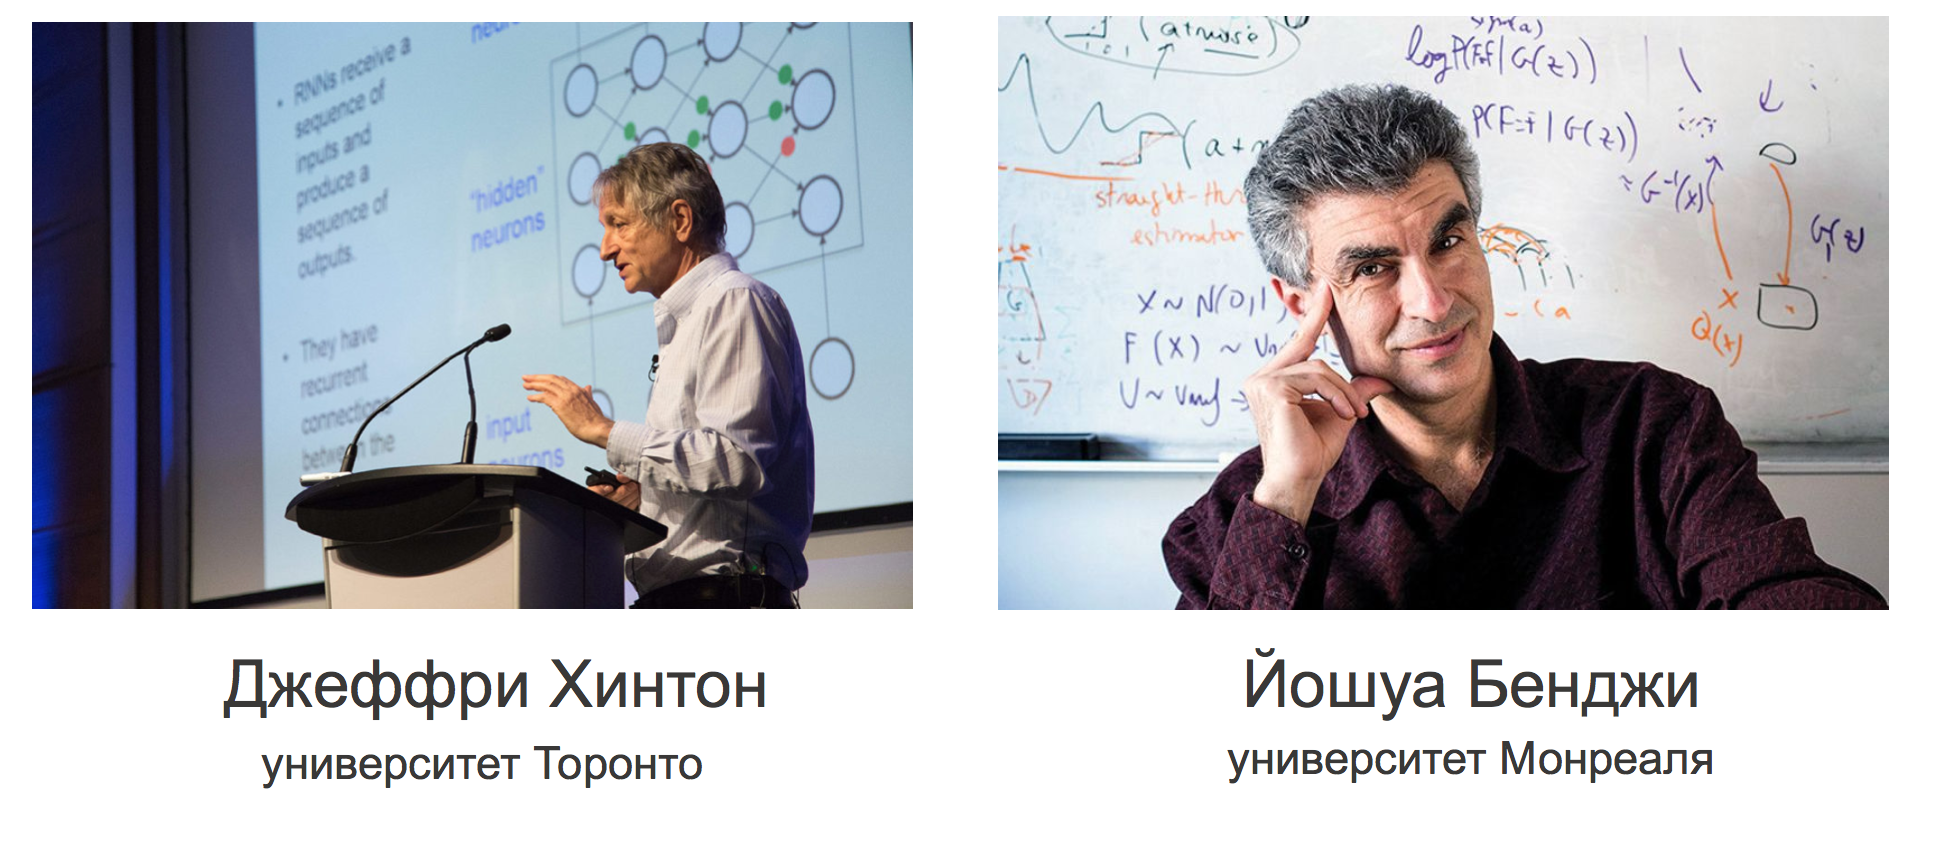
\includegraphics[width=0.9\paperwidth]{revolution.png}
\end{center}
\end{frame}


\begin{frame}{Революция}
\begin{wideitemize} 
\item 2005-2006 — группы Хинтона и Бенджи научились обучать глубокие нейросетки

\item Накопилось больше данных! Огромные данные! 

\item Компьютеры стали на порядки мощнее! Появились крутые GPU! 

\item На больших данных и мощностях заработали старые архитектуры

\item Появились новые алгоритмы, эвристики и подходы

\item Ящик Пандоры открыт! 
\end{wideitemize} 
\end{frame}

{
\usebackgroundtemplate{ 
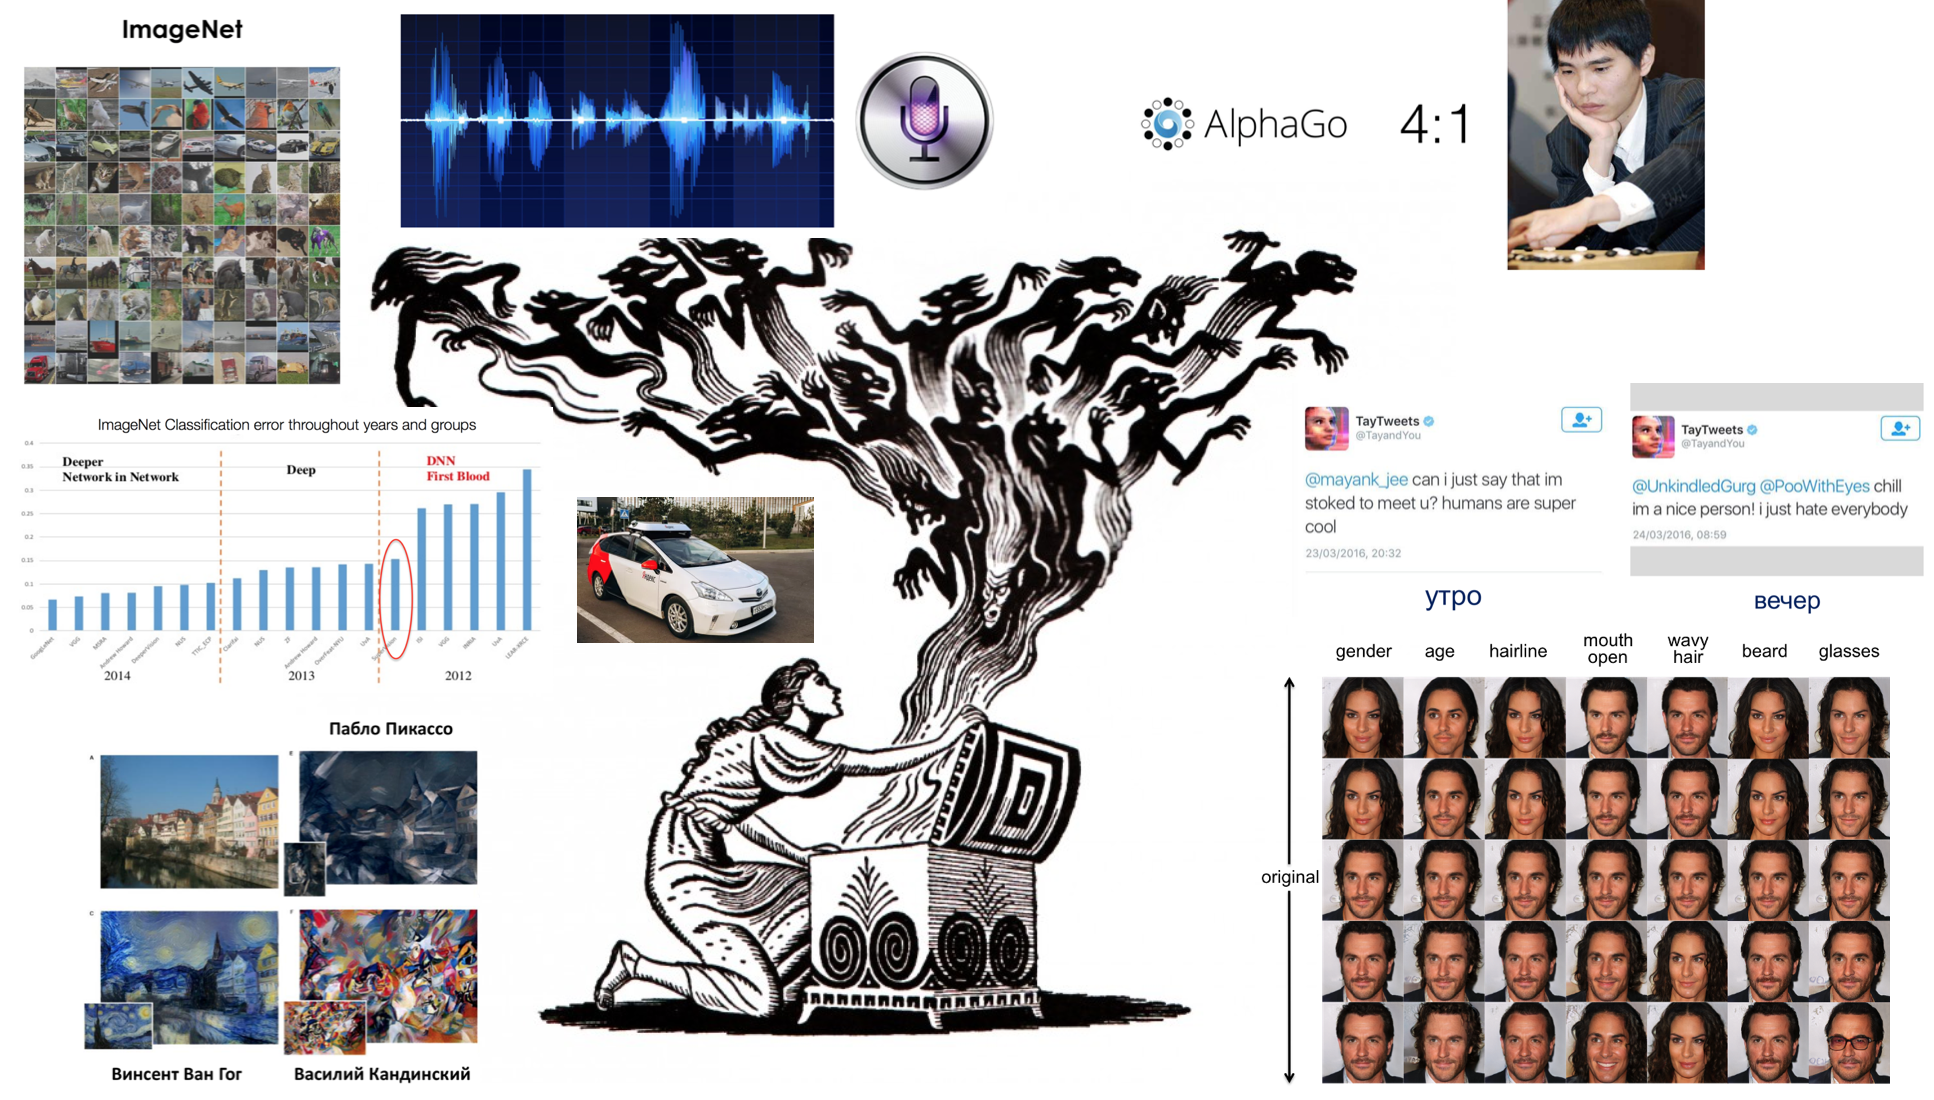
\includegraphics[width=\paperwidth]{pandora.png}}
\begin{frame}
\end{frame}
}


\begin{transitionframe}
	\begin{center}
		\Huge Линейные модели
	\end{center}
\end{transitionframe}


\begin{frame}{Линейная регрессия (постановка)}

\begin{wideitemize}
	\item  $y \in R$ — целевая переменная (рэйтинг фильма, стоимость квартиры, валютный курс и тп)
	\item  $X$ — признаки  
	\item  Модель: 
	\[
	 y = w_0 + w_1 x_1 + w_2 x_2 + \ldots + w_k x_k 
	\]
	\item  Нужно оценить $k+1$ параметр 
\end{wideitemize} 
\end{frame}

\begin{frame}{Линейная регрессия (векторная форма)}

\[
y = \begin{pmatrix} y_1 \\ y_2 \\ \ldots \\ y_n \end{pmatrix}  \qquad X = \begin{pmatrix} 1 & x_{11} & \ldots & x_{1k} \\ 1 & x_{21} & \ldots & x_{2k} \\ \ldots & \ddots & \ldots & \dots \\ 1 & x_{n1} & \ldots & x_{nk} \end{pmatrix}  \qquad  w = \begin{pmatrix} w_0 \\ w_1 \\ \ldots \\ w_k \end{pmatrix} 
\]

Модель: 

\[ 
y = Xw
\]

Прогноз: 

\[
\hat y = X \hat{w}
\]

\end{frame}


\begin{frame}{Линейная регрессия (функция потерь)}

Как тренировать модель? 

\[
L(w) = \frac{1}{n} \sum_{i=1}^n (w^T x_i - y_i)^2 = \frac{1}{n} ||Xw - y||^2 \to \min_{w}
\]

Существует аналитическое решение: 

\[
\hat w = (X^T X)^{-1} X^T y
\]

\end{frame}

{
	\usebackgroundtemplate{ 
		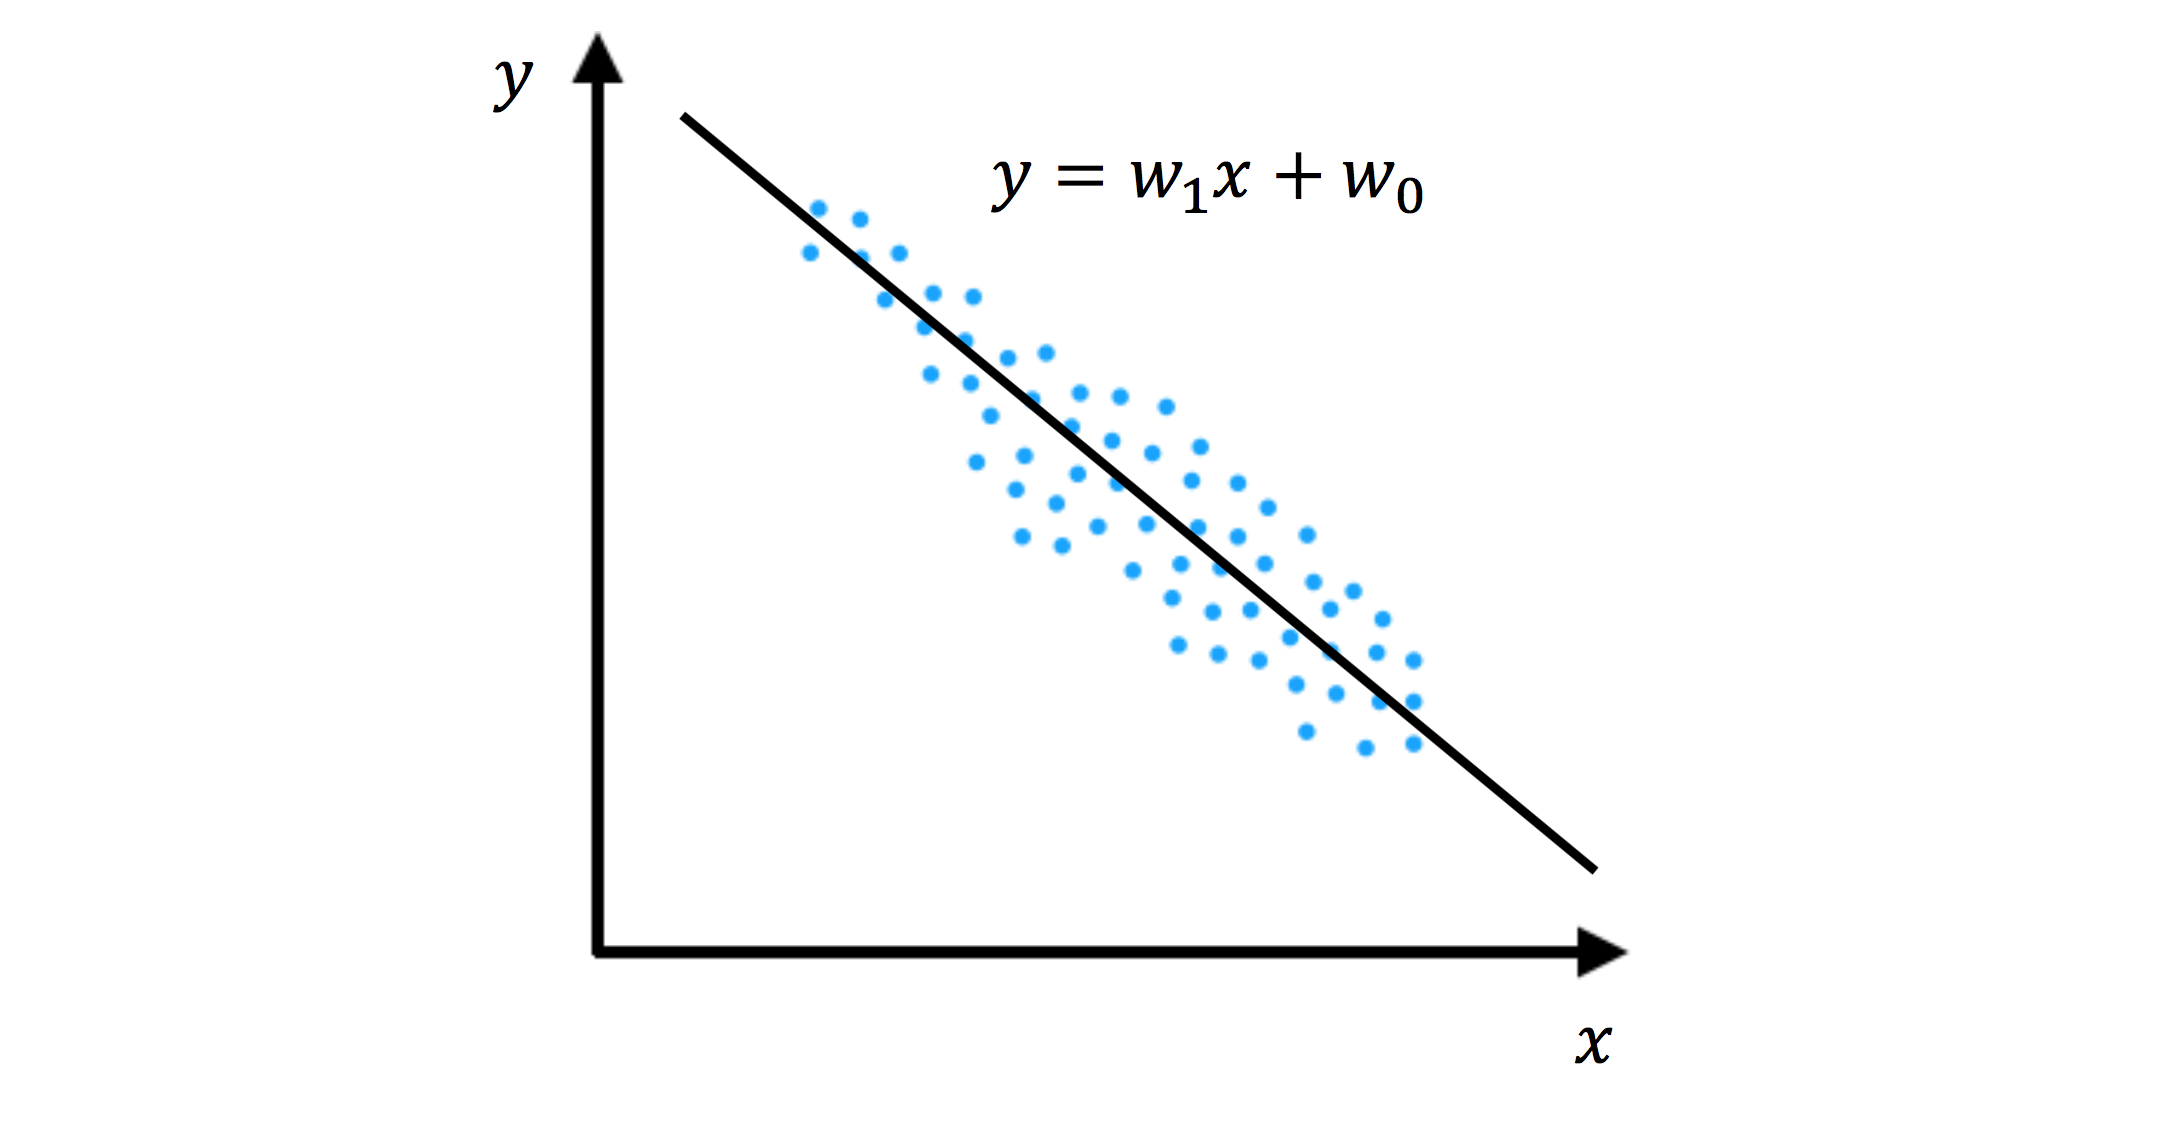
\includegraphics[width=\paperwidth]{regres.png}}
	\begin{frame}
\end{frame}
}


{
\usebackgroundtemplate{ 
	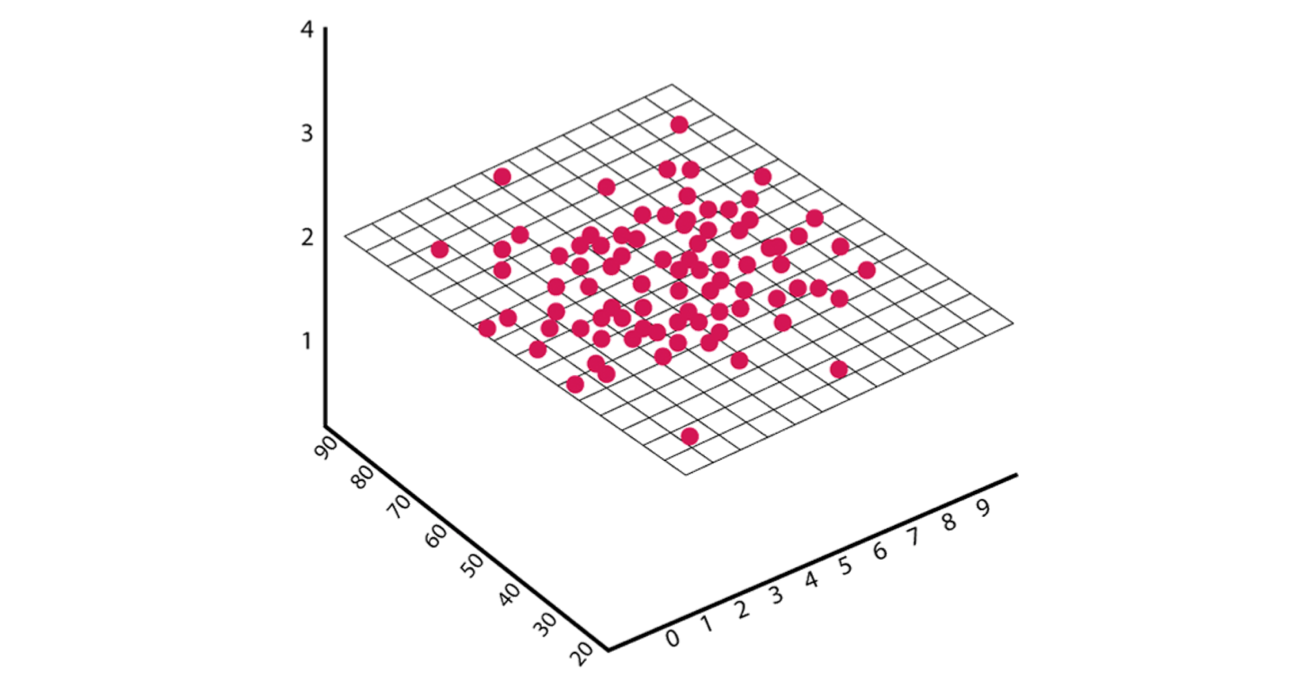
\includegraphics[width=\paperwidth]{reg3.png}}
\begin{frame}
\end{frame}
}

\begin{frame}{Резюме}
\begin{wideitemize}
	
	\item  Линейная регрессия очень простая для обучения модель
	
	\item $MSE$ можно использовать как функцию потерь для линейной регрессии, в такой ситуации существует аналитическое решение  
	
	\item Не для всех функция потерь бывает аналитическое решение, пример: $MAE$ 
	
	\[ MAE = \frac{1}{n} \sum_{i=1}^n |w^Tx_i - y_i| \]
	
	\item Поэтому на практике для обучения не используют аналитическое решение, выбирая более масшабируемые методы 
\end{wideitemize} 
\end{frame}


\begin{frame}{Классификация}

\begin{wideitemize}
	\item  $y \in \{0, 1 \}$ — целевая переменная (болен или здоров, кот или собака и тп)
	\item  $X$ — признаки  
	\item Хотим оценить
	\[
	P(y = 1 \mid X) = w_0 + w_1 x_1 + w_2 x_2 + \ldots + w_k x_k
	\]
	\item  Нужно оценить $k+1$ параметр 
\end{wideitemize} 
\end{frame}


\begin{frame}{Предсказание вероятностей}

\begin{wideitemize}
	\item Мы хотим оценить вероятность, но $w^T x_i$ не всегда лежит на отрезке $[0;1]$
\end{wideitemize}

\begin{center}
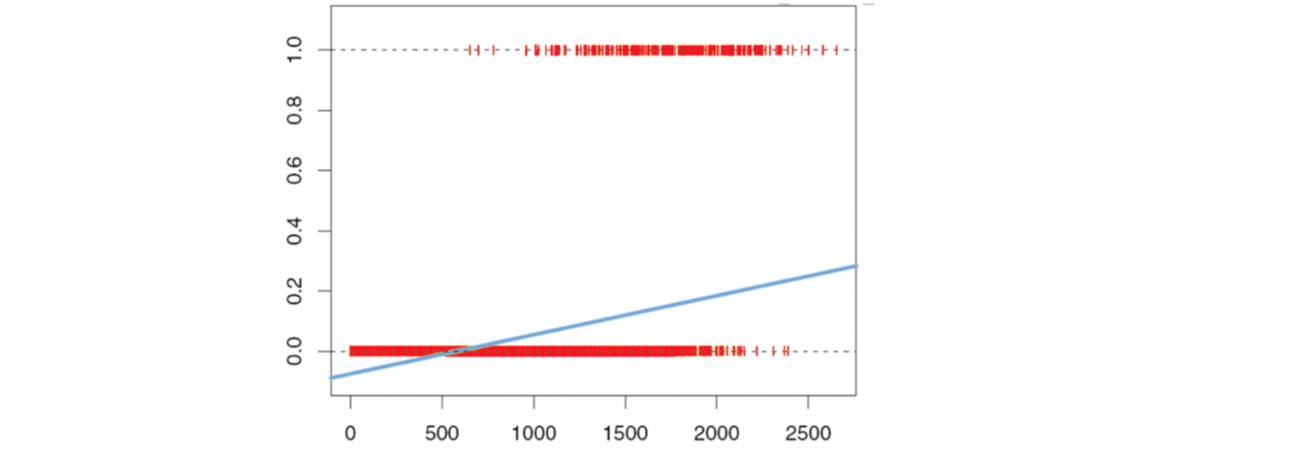
\includegraphics[width=\paperwidth]{logreg_problem.png}
\end{center}
\end{frame}

{
	\usebackgroundtemplate{ 
		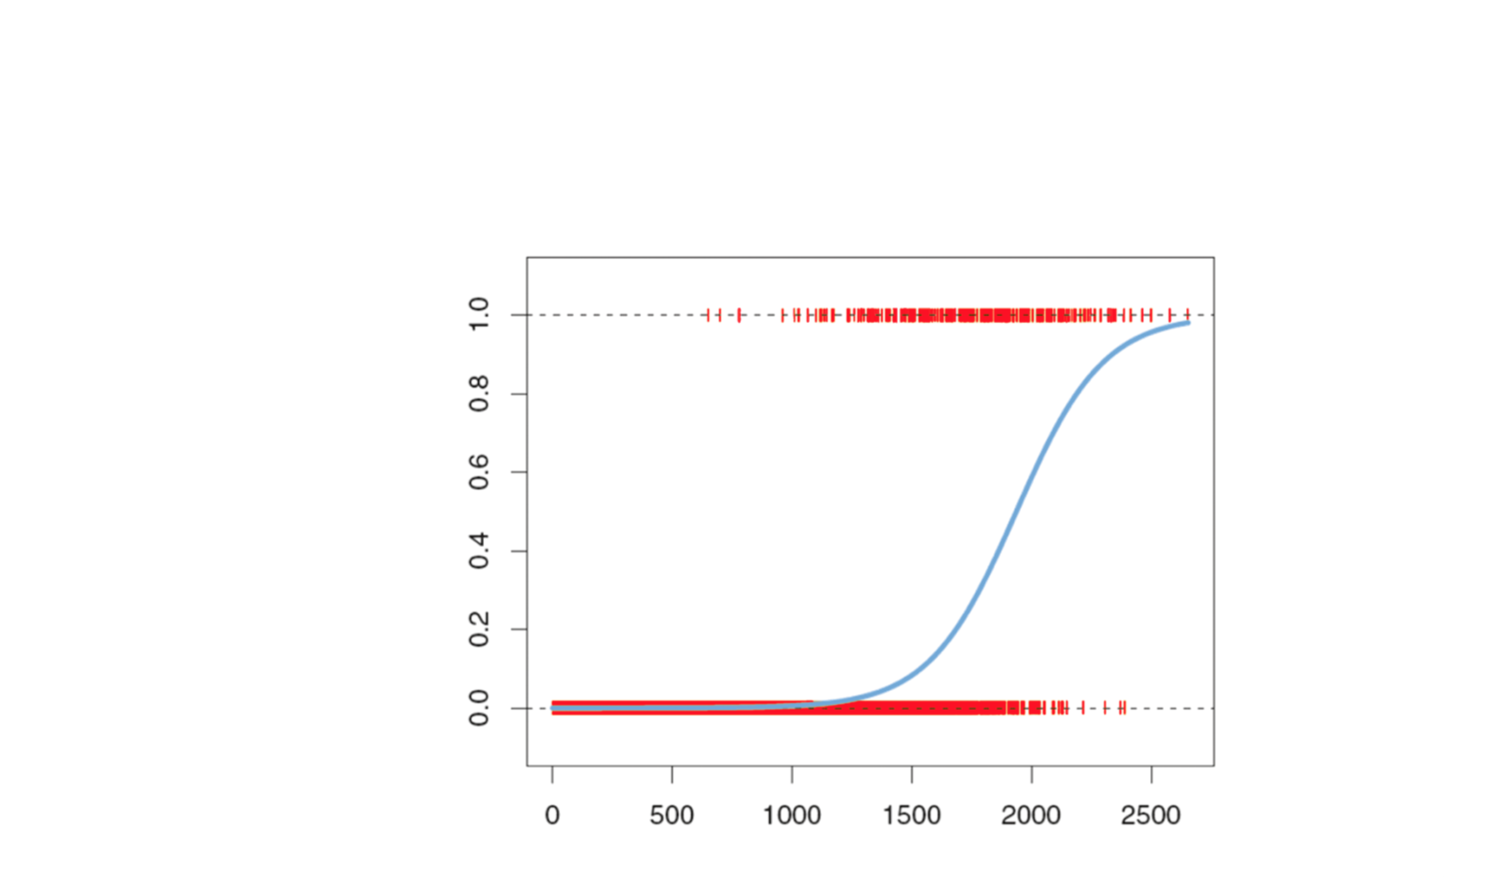
\includegraphics[width=0.9\paperwidth]{logreg_solveprob.png}}
	\begin{frame}
\end{frame}
}

\begin{frame}{Предсказание вероятностей}

\begin{wideitemize}
	\item Возьмём функцию $F$, которая переводит $w^Tx_i$ на отрезок $[0;1]$
	
	\[
		P(y = 1 \mid x) = F(w_0 + w_1 x_1 + w_2 x_2 + \ldots + w_k x_k)
	\]
	
	\item Чаще всего в качестве $F$ берут сигмоиду, логистическую функцию распределения
	
	\[
	P(y = 1 \mid x) = F(w^Tx) = \frac{ e^{w^Tx}}{1 + e^{w^Tx}} = \frac{1}{1 + e^{-w^Tx}}
	\]
	
	\item В её случае 
	
	\[
	\ln \frac{P(y=1 \mid X)}{P(y = 0 \mid X)} = w^Tx
	\]
\end{wideitemize}
\end{frame}


\begin{frame}{Логистическая регрессия (функция потерь)}

Как тренировать модель? Из метода максимального правдоподобия можно получить логистическую функцию потерь  

\[
L(w) = - \sum_{i=1}^n y_i \cdot \ln P(y_i = 1 \mid X) + (1 - y_i) \cdot \ln (1 - P(y_i = 1\mid X))
\]

Можно переписать

\[
L(w)  = - \sum_{i=1}^n \sum_{k \in \{0,1\}} [y_i = k] \cdot \ln \frac{e^{w^Tx}}{1 + e^{w^Tx}}
\]

\end{frame}


{
	\usebackgroundtemplate{ 
		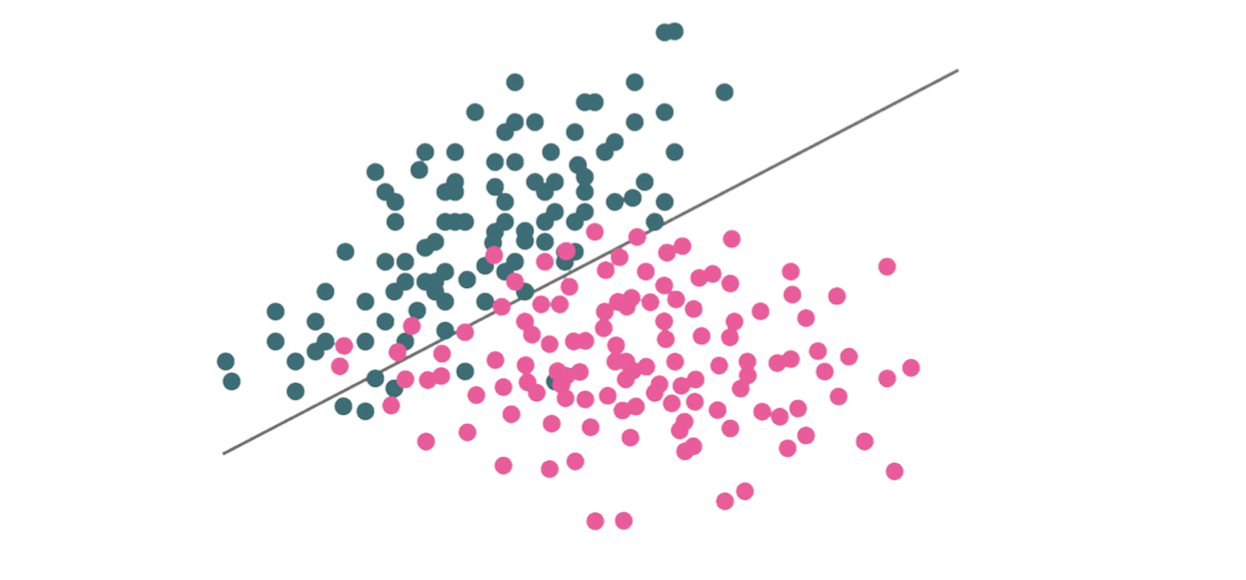
\includegraphics[width=\paperwidth]{logreg.png}}
	\begin{frame}
\end{frame}
}



\begin{frame}{Обобщение на много классов (softmax)}
	
Много классов, $y \in {1, \ldots, K}$
	
\begin{equation*}
\begin{aligned}
(w_1^T x, &\ldots, w_K^Tx) \\
&\Downarrow \\
(e^{z_1}, &\ldots, e^{z_K}) \\
&\Downarrow \\
\left(\frac{e^{z_1}}{\sum_{k=1}^K e^{z_k}}\right., &\ldots,\left. \frac{e^{z_K}}{\sum_{k=1}^K e^{z_k}}  \right)
\end{aligned}
\end{equation*}

Потери (кросс-энтропия): 

\[
L(w) - \sum_{i=1}^n \sum_{k=1}^K [y_i = k] \cdot \ln \frac{e^{w_k^Tx_i}}{\sum_{j=1}^{K} e^{w_j^Tx_i}}
\]
\end{frame}

\begin{transitionframe}
	\begin{center}
		\Huge Переобучения и регуляризация
	\end{center}
\end{transitionframe}


\begin{frame}{Оценка качества модели}
\begin{wideitemize}
	\item На тренировочной выборке модель показывает долю правильных ответов $80\%$
	\item Означает ли это, что на новых данных модель будет работать также хорошо? 
	\item Обладает ли модель обобщающими способностями? 
\end{wideitemize}
\end{frame}


\begin{frame}{Отложенная выборка}
\begin{center}
	
\includegraphics[width=0.7\paperwidth]{holdout_set.png}
\end{center}

\begin{wideitemize}
	\item На тренировочной выборке учим модель
	\item Для проверки качества используем отложенную (тестовую) выборку
	\item Итоговая оценка качества зависит от разбиения 
\end{wideitemize}
\end{frame}

\begin{frame}{Кросс-валидация}
\begin{center}
	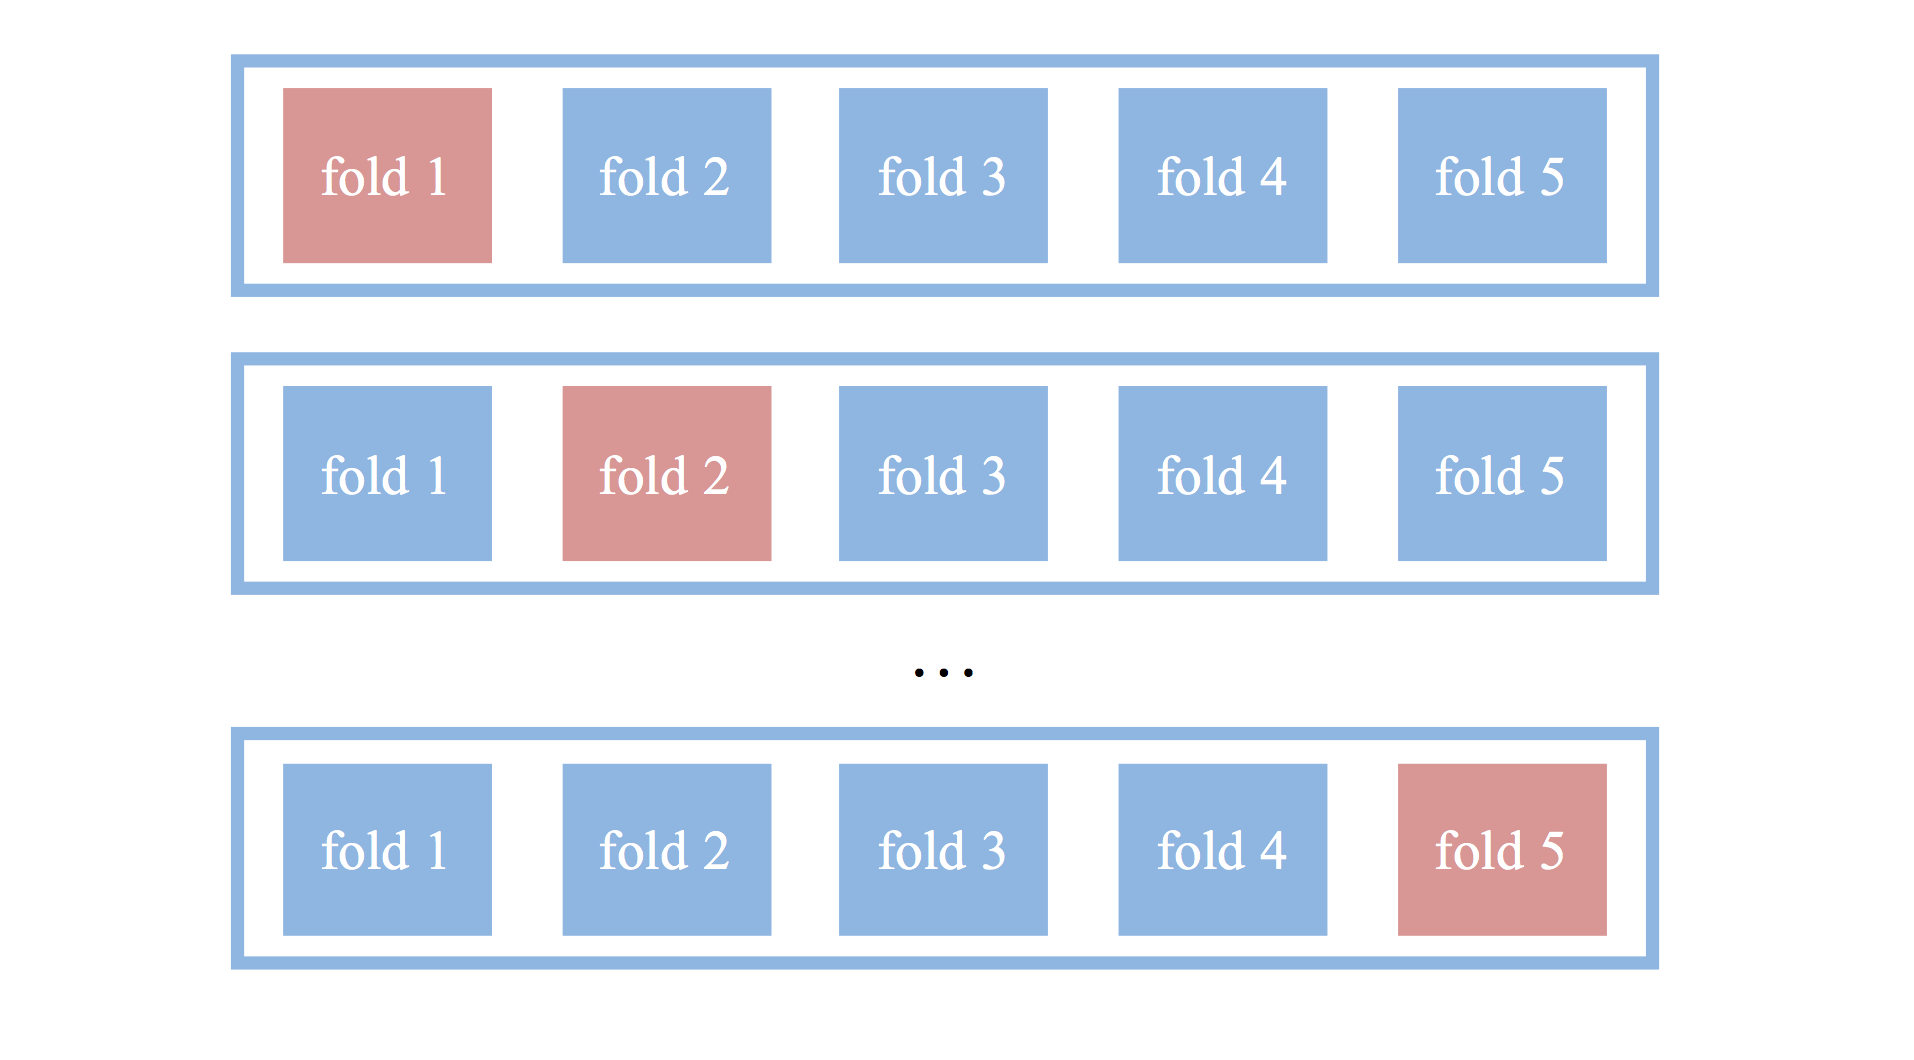
\includegraphics[width=0.6\paperwidth]{cross_validation.png}
\end{center}

\begin{wideitemize}
	\item Нужно оценить $K$ моделей, нет зависимости от разбиения
	\item Для нейросеток обычно не используют, потому что долго
\end{wideitemize}
\end{frame}


\begin{frame}{Переобучение}
\begin{center}
	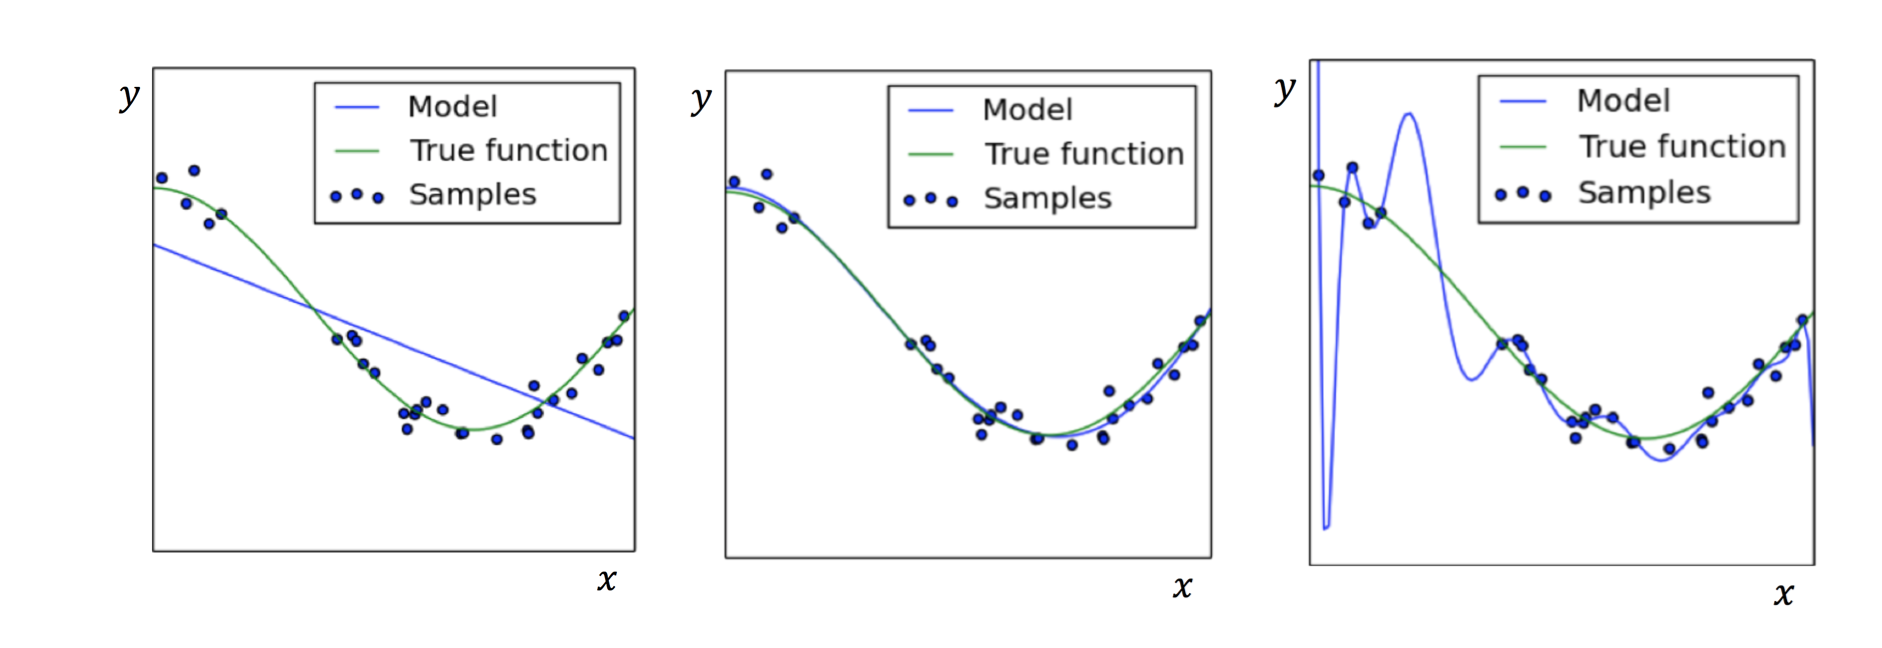
\includegraphics[width=0.9\paperwidth]{overfit.png}
\end{center}
\end{frame}

\begin{frame}{Регуляризация}
\begin{wideitemize}
	\item В хорошей модели: $(0.634, 0.918, -0.626)$
	\item В переобученной модели: $(130.0, -525.8, \ldots, 102.6)$
	\item Мысль: оштрафовать модель за излишне большие веса, это уберёт изгибы и сделает её проще
	
	\[
	L(w) + \lambda \cdot R(w) \to \min_{w}
	\]
	
	\item В общем случае регуляризаторы помогают получить решение с желаемыми нам свойствами
\end{wideitemize}
\end{frame}


\begin{frame}{$l_2$ регуляризация}

\[L(w) + \lambda \cdot  \sum w_i^2  \to \min_{w}\]

Задача оптимизации эквивалентна:

\[
\begin{cases} 
L(w) \to \min_{w} \\
\sum w_i^2 \le C \\
\end{cases}
\]

\begin{center}
	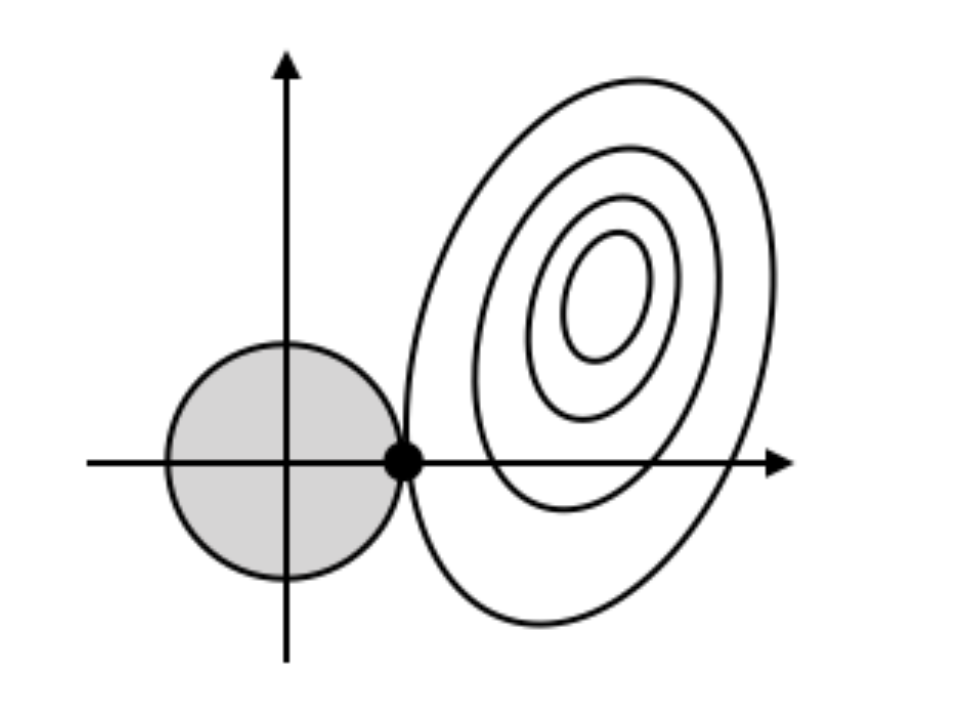
\includegraphics[width=0.35\paperwidth]{l2reg.png}
\end{center}
\end{frame}



\begin{frame}{$l_1$ регуляризация}

\[L(w) + \lambda \cdot  \sum w_i|  \to \min_{w}\]

Задача оптимизации эквивалентна:

\[
\begin{cases} 
L(w) \to \min_{w} \\
\sum |w_i| \le C \\
\end{cases}
\]

\begin{center}
	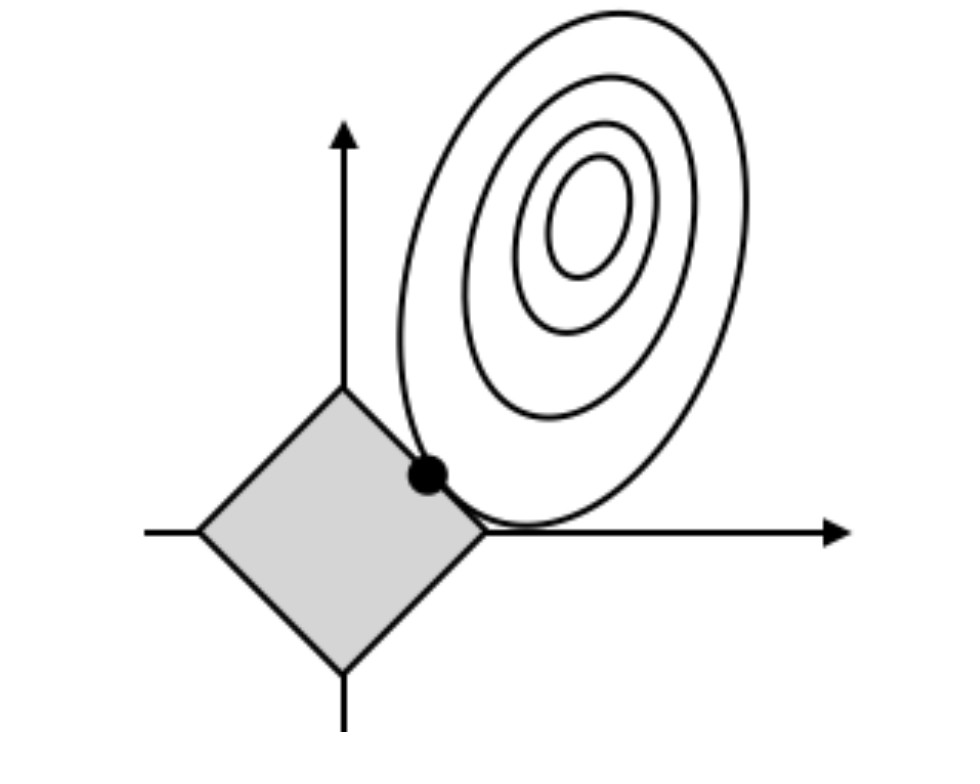
\includegraphics[width=0.35\paperwidth]{l1reg.png}
\end{center}
\end{frame}



\begin{frame} 
\begin{wideitemize}
	\item Регуляризация помогает избежать переобучения, ситуации, когда модель излишне подробно вылизывает данные и настраивается на шум, вместо выделения сигнала
	\item Нейросетки довольно сложные модели, включающие огромное количество параметров, на маленькой выборке их довольно легко переобучить 
	\item Для борьбы с переобучением мы будем использовать как уже знакомые нам регуляризаторы, так и новые техники
\end{wideitemize}
\end{frame}



\begin{transitionframe}
	\begin{center}
		\Huge Градиентный спуск
	\end{center}
\end{transitionframe}

\begin{frame}{Как обучать?}
\begin{wideitemize}
	\item «Тренировка» — поиск оптимальных $W$ 
	\item «Оптимальных» — минимизирующих какой-то функционал 
	\item Какими бывают функционалы: MSE, MAE, Logloss
	\item Как оптимизировать: градиентный спуск! 
\end{wideitemize} 
\end{frame}

\begin{frame}[fragile]{Градиентный спуск (GD)}
Проблема оптимизации: 

\[   
L(w) = \sum_{i=1}^n L(w, x_i, y_i) \to \min_{w}
\]

Инициализация $w_0$ 
\mint{python}{while True:}
\hspace{15pt} $g_t = \frac{1}{n}\sum_{i=1}^n  \nabla L(w, x_i, y_i)$ \\
\pgr{\hspace{15pt}} $w_t = w _{t-1} - \eta_t \cdot g_t $ \\
\pgr{\hspace{15pt} if} $||w_t - w_{t-1}|| < \varepsilon:$ \\
\pgr{\hspace{30pt} break}
\end{frame}


\begin{frame}{Градиентный спуск}
\begin{center}
	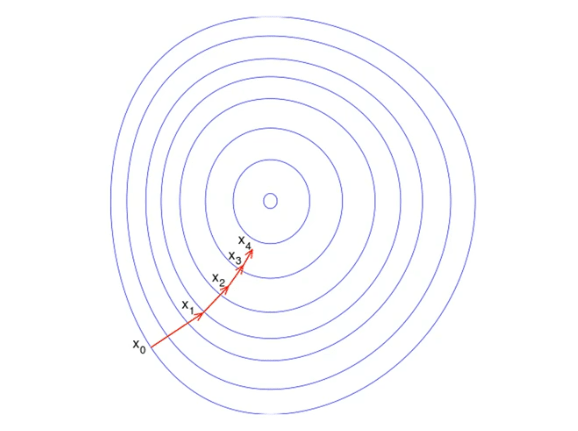
\includegraphics[width=.6\linewidth]{2dgrad.png}
\end{center}
\end{frame}


\begin{frame}[fragile]{Стохастический градиентный спуск (SGD)}
Проблема оптимизации: 

\[   
L(w) = \sum_{i=1}^n L(w, x_i, y_i) \to \min_{w}
\]


Инициализация $w_0$ 
\mint{python}{while True:}
\hspace{15pt} рандомно выбрали $i$ \\
\pgr{\hspace{15pt}} $g_t = \nabla L(w_{t-1}, x_i, y_i)$ \\
\pgr{\hspace{15pt}} $w_t = w _{t-1} - \eta_t \cdot g_t  $ \\
\pgr{\hspace{15pt} if} $||w_t - w_{t-1}|| < \varepsilon:$ \\
\pgr{\hspace{30pt} break}
\end{frame}


\begin{frame}{Стохастический градиентный спуск (SGD)}
\begin{columns}[T] %
	\begin{column}{.4\textwidth}
		\resizebox{0.95\linewidth}{!}{
			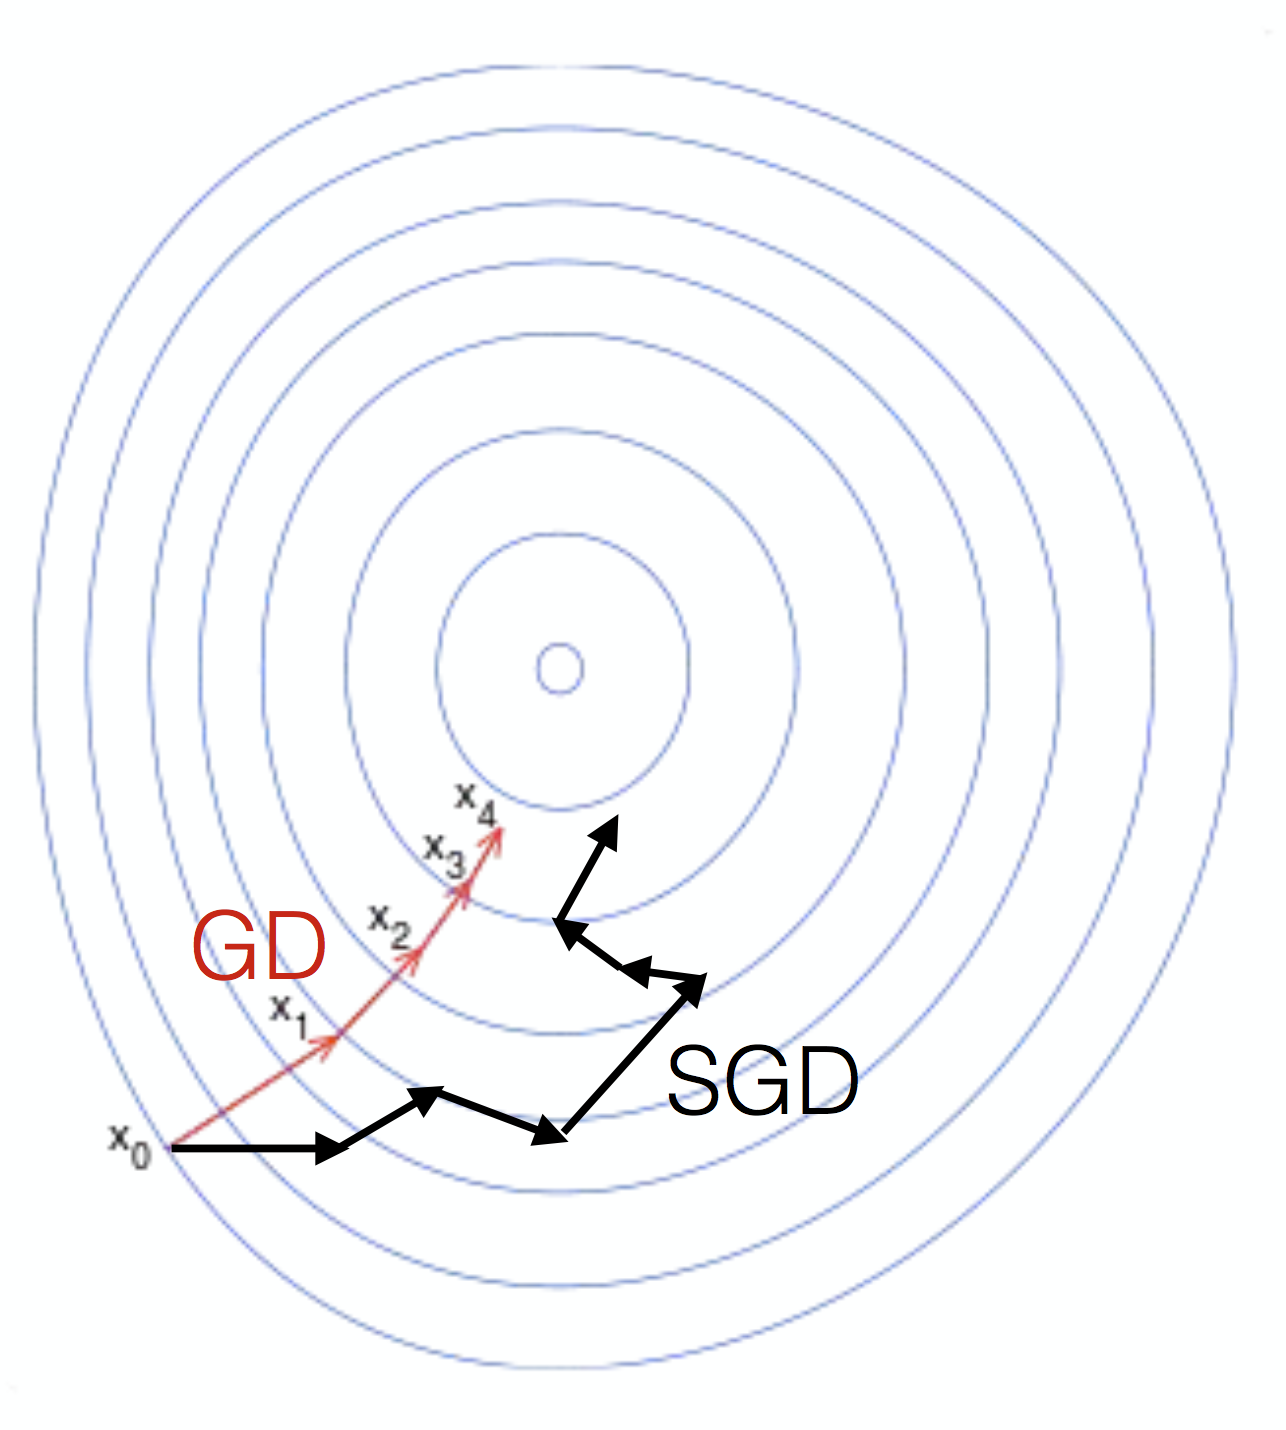
\includegraphics{st2grad.png}
		}
	\end{column}%
	\hfill%
	\begin{column}{.6\textwidth}
		\begin{wideitemize}
			\item И для GD и для SGD нет гарантий глобального минимума, сходимости
			\item SGD быстрее,на каждой итерации используется только одно наблюдение
			\item Для SGD спуск очень зашумлён 
			\item  GD: $O(n)$, SGD: $O(1)$
			\item Скорость обучения надо подбирать аккуратно, если она будет большой, мы можем скакать вокруг минимума, если маленькой - вечно ползти к нему
		\end{wideitemize}
	\end{column}%
\end{columns}
\end{frame}


\begin{frame}[fragile]{Mini-bath SGD}
Проблема оптимизации: 

\[   
L(w) = \sum_{i=1}^n L(w, x_i, y_i) \to \min_{w}
\]

Инициализация $w_0$ 
\mint{python}{while True:}
\pgr{\hspace{15pt}} рандомно выбрали $m < n$ индексов \\
\pgr{\hspace{15pt}} $g_t =\frac{1}{m}\sum_{i=1}^m  \nabla L(w, x_i, y_i)$ \\
\pgr{\hspace{15pt}} $w_t = w _{t-1} - \eta_t \cdot g_t   $ \\
\pgr{\hspace{15pt} if} $||w_t - w_{t-1}|| < \varepsilon:$ \\
\pgr{\hspace{30pt} break}
\end{frame}


\begin{frame}{Momentum SGD}

Мы считали на каждом шаге градиент по формуле  \[g_t =\frac{1}{m}\sum_{i=1}^m  \nabla L(w, x_i, y_i).\] После шага мы забывали его. {\color{red} А давайте попробуем помнить направление:} 

\begin{equation*}
	\begin{aligned}
	h_t &= \alpha \cdot h_{t-1} + \eta_t \cdot g_t \\
	w_t &= w_{t-1} - h_t
	\end{aligned}	
\end{equation*}

\begin{itemize}
	\item Движение поддерживается в том же направлении, что и на предыдущем шаге
	\item Нет резких изменений направления движения.
	\item Обычно $\alpha = 0.9$.
\end{itemize}
\end{frame}


\begin{frame}{Momentum SGD}
\begin{wideitemize}
	\item Бежим с горки и всё больше ускоряемся в том направлении, в котором были направлены сразу несколько предыдущих градиентов, но при этом движемся медленно там, где градиент постоянно меняется
	\item Хотелось бы не просто бежать с горы, но и хотя бы на полшага смотреть себе под ноги, чтобы внезапно не споткнуться $\Rightarrow$ давайте смотреть на градиент в будущей точке
	\item Согласно методу моментов $\alpha h_{t-1}$ точно будет использоваться при шаге, давайте искать $\nabla L(w_{t-1} - \alpha \cdot h_{t-1})$.
\end{wideitemize}
\end{frame}


\begin{frame}{Nesterov Momentum SGD}
\begin{center}
	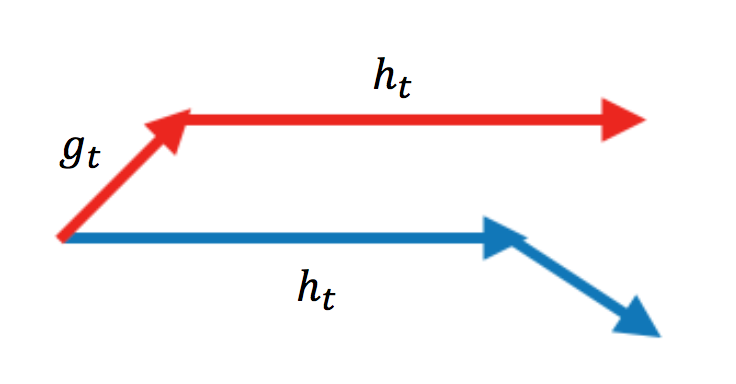
\includegraphics[width=.4\linewidth]{nesterov.png}
\end{center}

\begin{equation*}
\begin{aligned}
h_t &= \alpha \cdot h_{t-1} + \eta_t \nabla L(w_{t-1} - \alpha \cdot h_{t-1}) \\
w_t &= w_{t-1} - h_t
\end{aligned}	
\end{equation*}
\end{frame}


\begin{frame}{Momentum SGD}
\begin{wideitemize}
	\item Может сложиться, что некоторые веса уже близки к своим локальным минимумам, по этим координатам надо двигаться медленнее, а по другим быстрее $\Rightarrow$ {\color{red} адаптивные методы градиентного спуска }

	\item Шаг изменения должен быть меньше у тех параметров, которые в большей степени варьируются в данных, и больше у тех, которые менее изменчивы 
\end{wideitemize}
\end{frame}


\begin{frame}{AdaGrad}
\begin{equation*}
\begin{aligned}
G_t^j &= G_{t-1}^j + g_{tj}^2 \\
w_t^j &= w_{t-1}^j - \frac{\eta_t}{\sqrt{G_t^j + \varepsilon}} \cdot g_t^j
\end{aligned}	
\end{equation*}

\begin{itemize}
	\item  $g_t^j$ — градиент по $j-$ому параметру
	\item своя скорость обучения для каждого параметра
	\item обычно $\eta_t = 0.01$, этот параметр не имеет значения
	\item $G_t^j$ всегда увеличивается, из-за этого обучение может рано останавливаться
\end{itemize}
\end{frame}


\begin{frame}{RMSprop}
\begin{equation*}
\begin{aligned}
G_t^j &= \alpha \cdot G_{t-1}^j + (1 - \alpha) \cdot g_{tj}^2 \\
w_t^j &= w_{t-1}^j - \frac{\eta_t}{\sqrt{G_t^j + \varepsilon}} \cdot g_t^j
\end{aligned}	
\end{equation*}

\begin{itemize}
	\item Обычно $ \alpha = 0.9$
	\item Скорость обучения адаптируется к последнему сделанному шагу
\end{itemize}
\end{frame}


\begin{frame}{Adam}
\begin{equation*}
\begin{aligned}
h_t^j &= \beta_1 \cdot h_{t-1}^j + (1 - \beta_1) \cdot g_{tj} \\
G_t^j &= \beta_2 \cdot G_{t-1}^j + (1 - \beta_2) \cdot g_{tj}^2 \\
w_t^j &= w_{t-1}^j - \frac{\eta_t}{\sqrt{G_t^j + \varepsilon}} \cdot h_t^j
\end{aligned}	
\end{equation*}

\begin{itemize} 
Комбинируем momentum и индивидуальные скорости обучения
\end{itemize}
\end{frame}


\begin{frame}{Подведём итоги}
\begin{wideitemize}
	\item Momentum SGD сохраняет направление шага и позволяет добиваться более быстрой сходимости
	
	\item  Адаптивные методы позволяют находить индивидуальную скорость обучения для каждого параметра
	
	\item Adam комбинирует в себе оба подхода
\end{wideitemize}
\end{frame}


\begin{transitionframe}
	\begin{center}
		\Huge Перцептрон 
	\end{center}
\end{transitionframe}


\begin{frame}{Перцептрон}
\begin{itemize}
	\item  {\color{blue} Перцептрон —} древняя штука, придуманная Розенблатом в $1950$-е годы.
\end{itemize}
\end{frame}



\begin{frame}{Перцептрон Розенблатта}
\begin{center}
	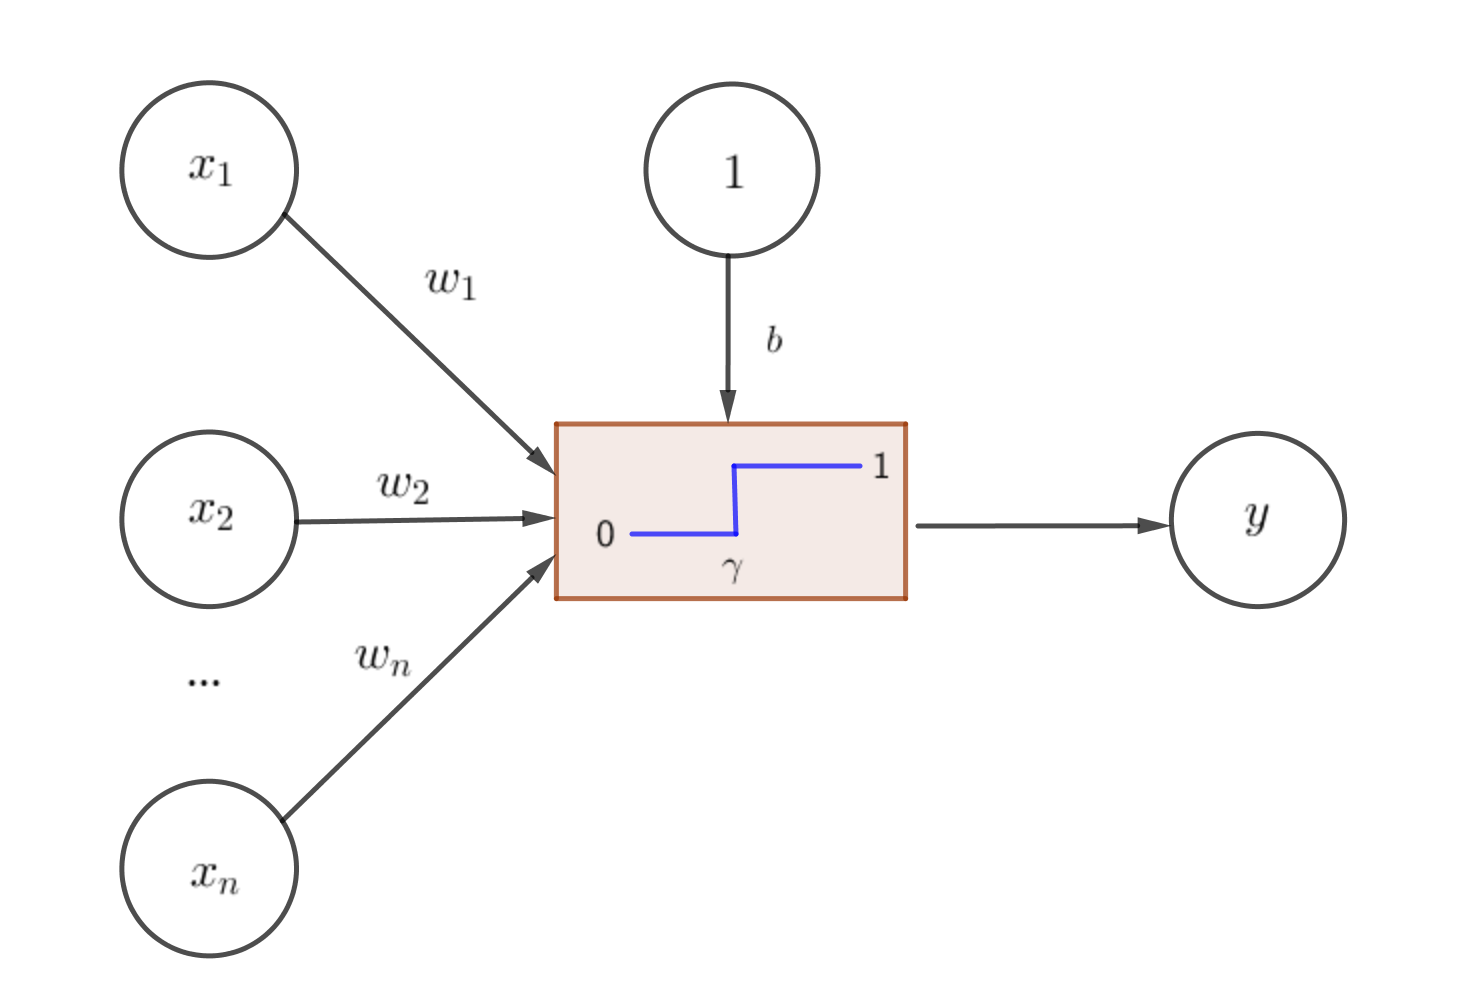
\includegraphics[width=0.55\paperwidth]{neuron_1.png}
\end{center}
\[
y = \begin{cases}
1, \text{ если } \sum w_i x_i \ge \gamma \\
0, \text{ если } \sum w_i x_i < \gamma \\
\end{cases}
\]
\end{frame}


\begin{frame}{Немного иной перцептрон Розенблатта}
\begin{center}
	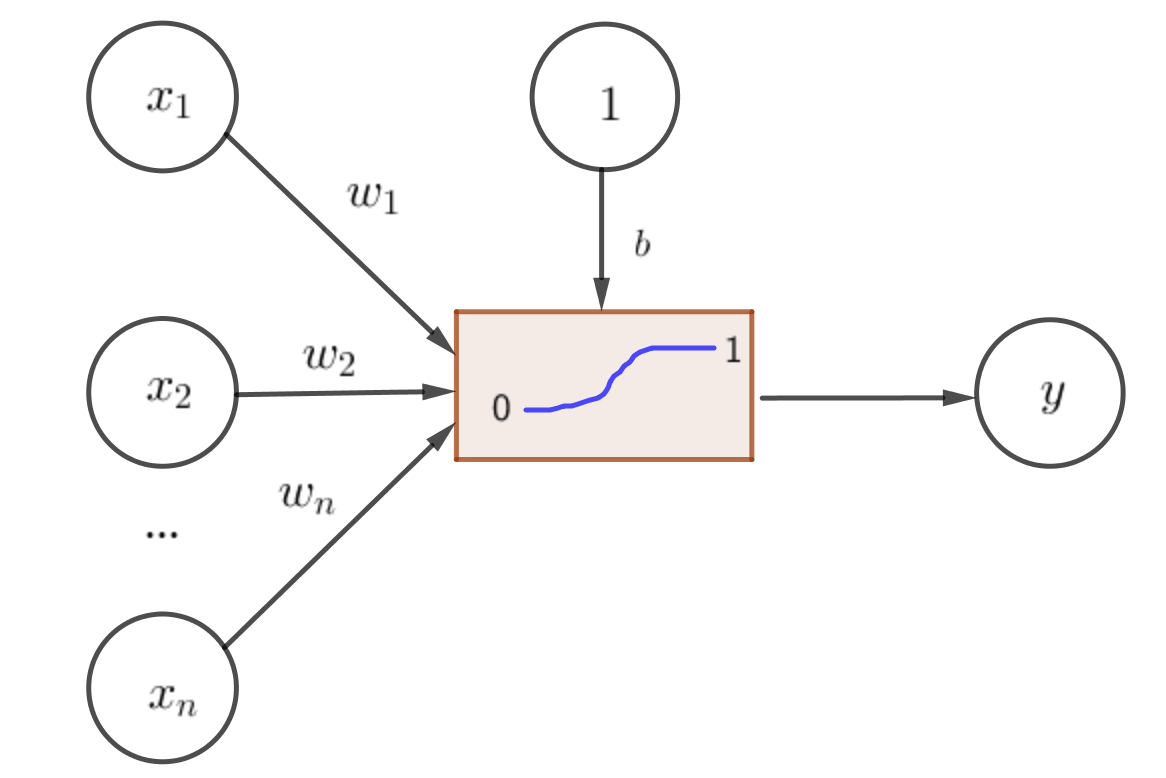
\includegraphics[width=0.55\paperwidth]{neuron_2.png}
\end{center}
\end{frame}


\begin{frame}{Функция активации}
\begin{center}
	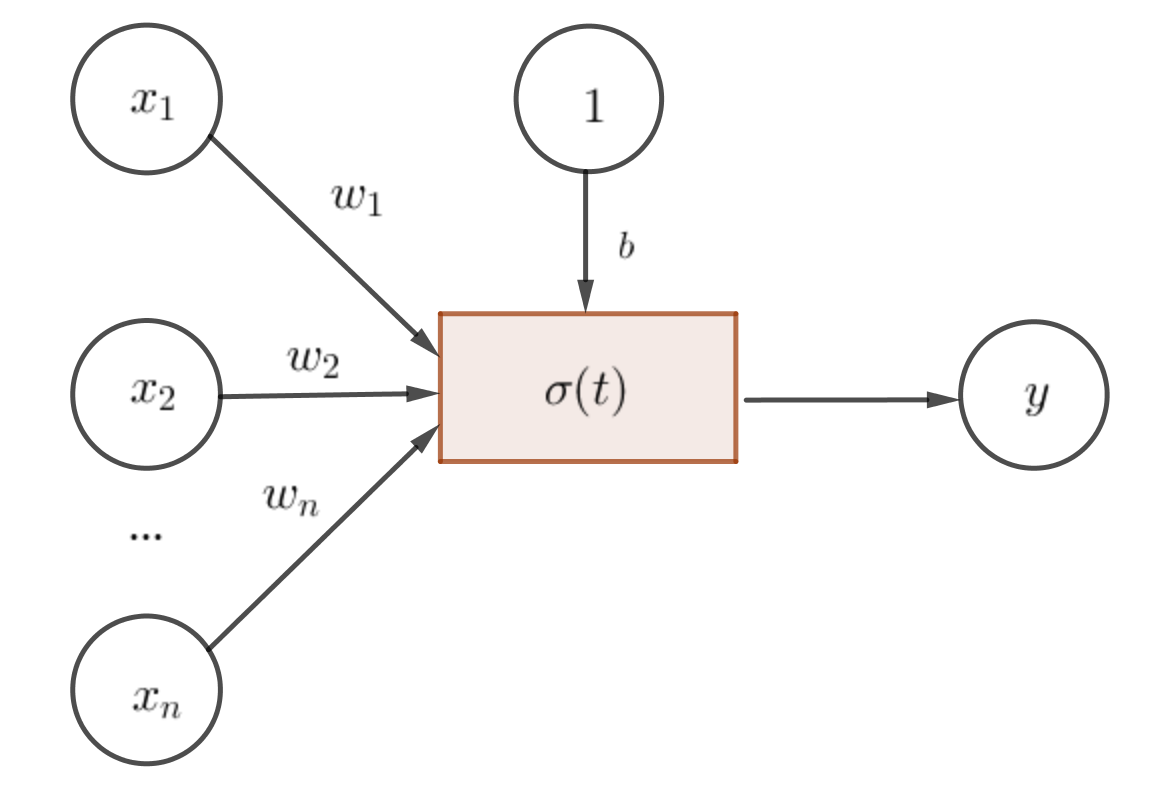
\includegraphics[width=0.51\linewidth]{neuron_3.png}
\end{center}
\begin{itemize}
	\item Функция активации $\sigma(t)$ вносит нелинейность, она может быть любой
\end{itemize}
\end{frame}


\begin{frame}{Линейная регрессия}
\begin{columns}[T] 
	\begin{column}{.45\textwidth}
		\begin{center}
			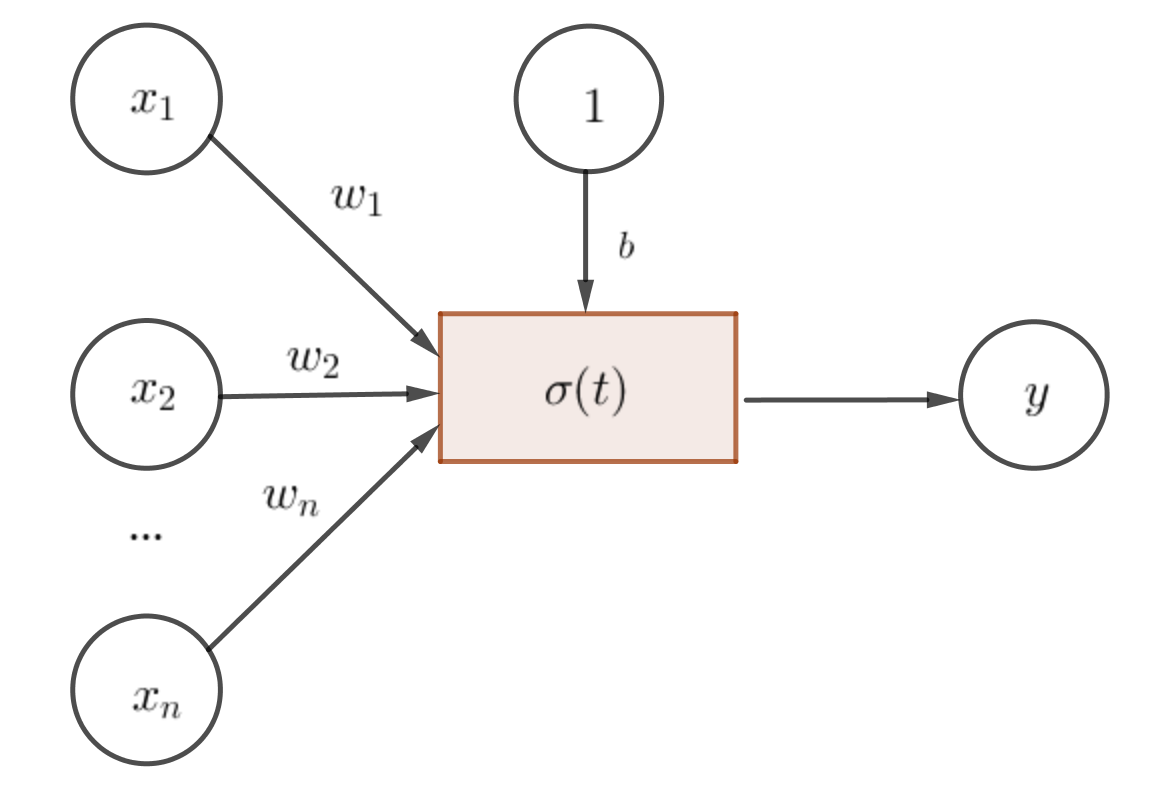
\includegraphics[width=0.99\linewidth]{neuron_3.png}
		\end{center}
	\end{column}%
	\hfill%
	\begin{column}{.55\textwidth}
		Нейрон с линейной функции активации~—   это линейная регрессия... 
		\begin{equation*}
		\begin{aligned}
		& \sigma(t) = t \\
		& y= b + w_1 x_1 + \ldots + w_n x_n \\
		\end{aligned}
		\end{equation*}
	\end{column}%
\end{columns}
\end{frame}


\begin{frame}{Логистическая регрессия}
\begin{columns}[T] 
	\begin{column}{.45\textwidth}
		\begin{center}
			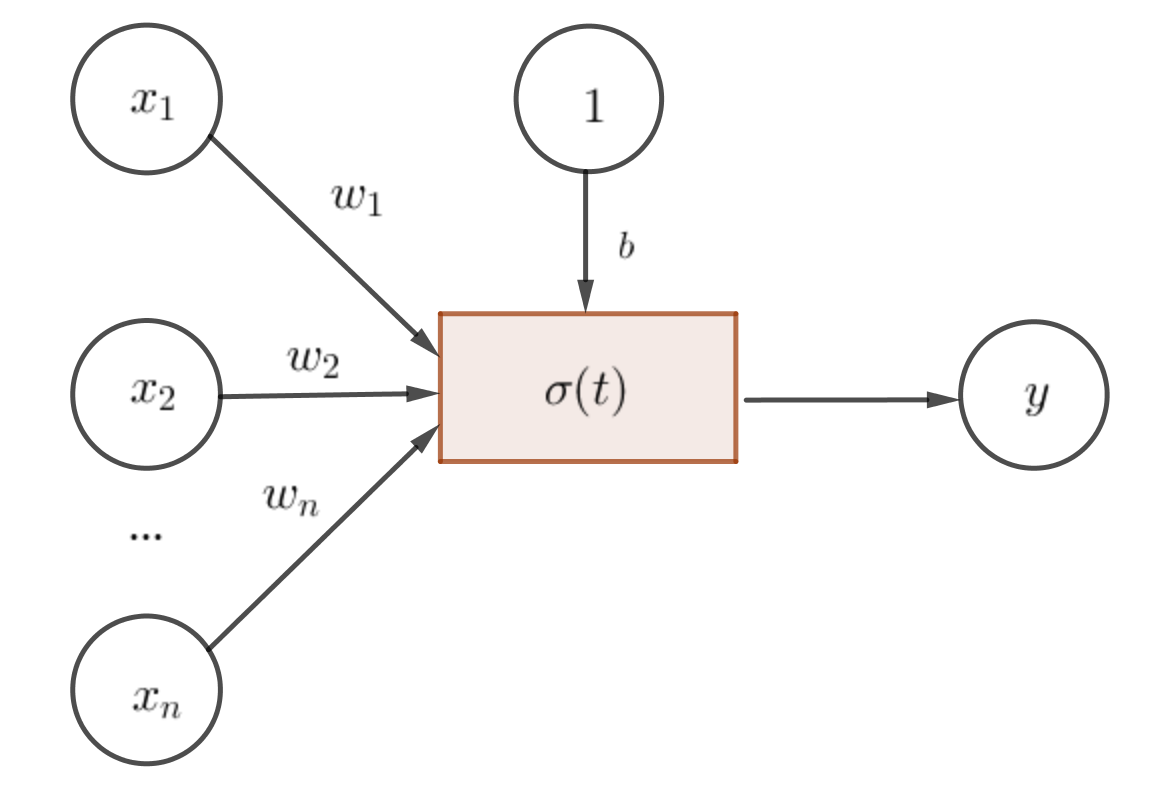
\includegraphics[width=0.99\linewidth]{neuron_3.png}
		\end{center}
	\end{column}%
	\hfill%
	\begin{column}{.55\textwidth}
		Нейрон с сигмоидом в качестве функции активации — это логистическая регрессия... 
		\begin{equation*}
		\begin{aligned}
		& \sigma(t) = \frac{1}{1 + e^{-t}} \\
		& P(y = 1 \mid x) = \sigma(b + w_1 x_1 + \ldots + w_n x_n) \\
		\end{aligned}
		\end{equation*}
	\end{column}%
\end{columns}
\end{frame}


\begin{frame}{Функция активации}
\begin{center}
	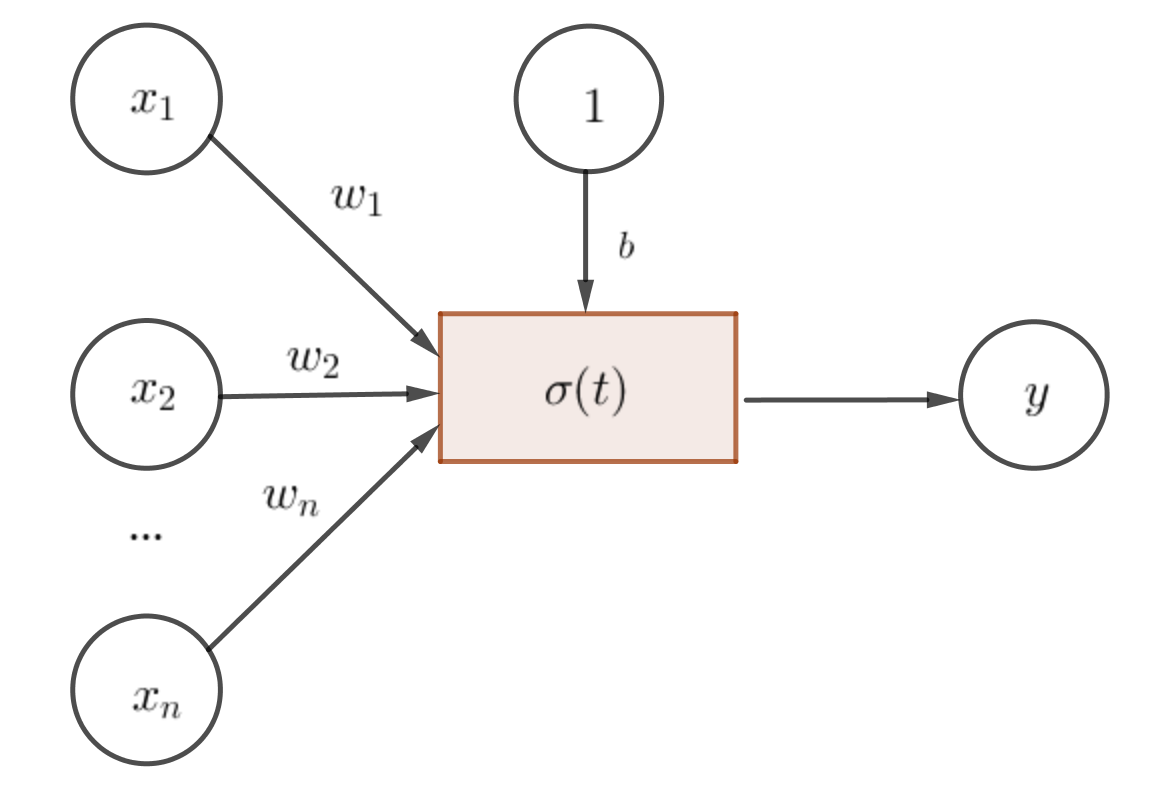
\includegraphics[width=0.51\linewidth]{neuron_3.png}
\end{center}
\begin{equation*}
\begin{aligned}
y &= \sigma(w_0 + w_1 \cdot x_1 + \ldots + w_n \cdot x_n) = \sigma(X w) \\ 
h & = X w
\end{aligned}
\end{equation*}
\end{frame}


\begin{frame}{Две регрессии скрепили третьей}
\begin{center}
	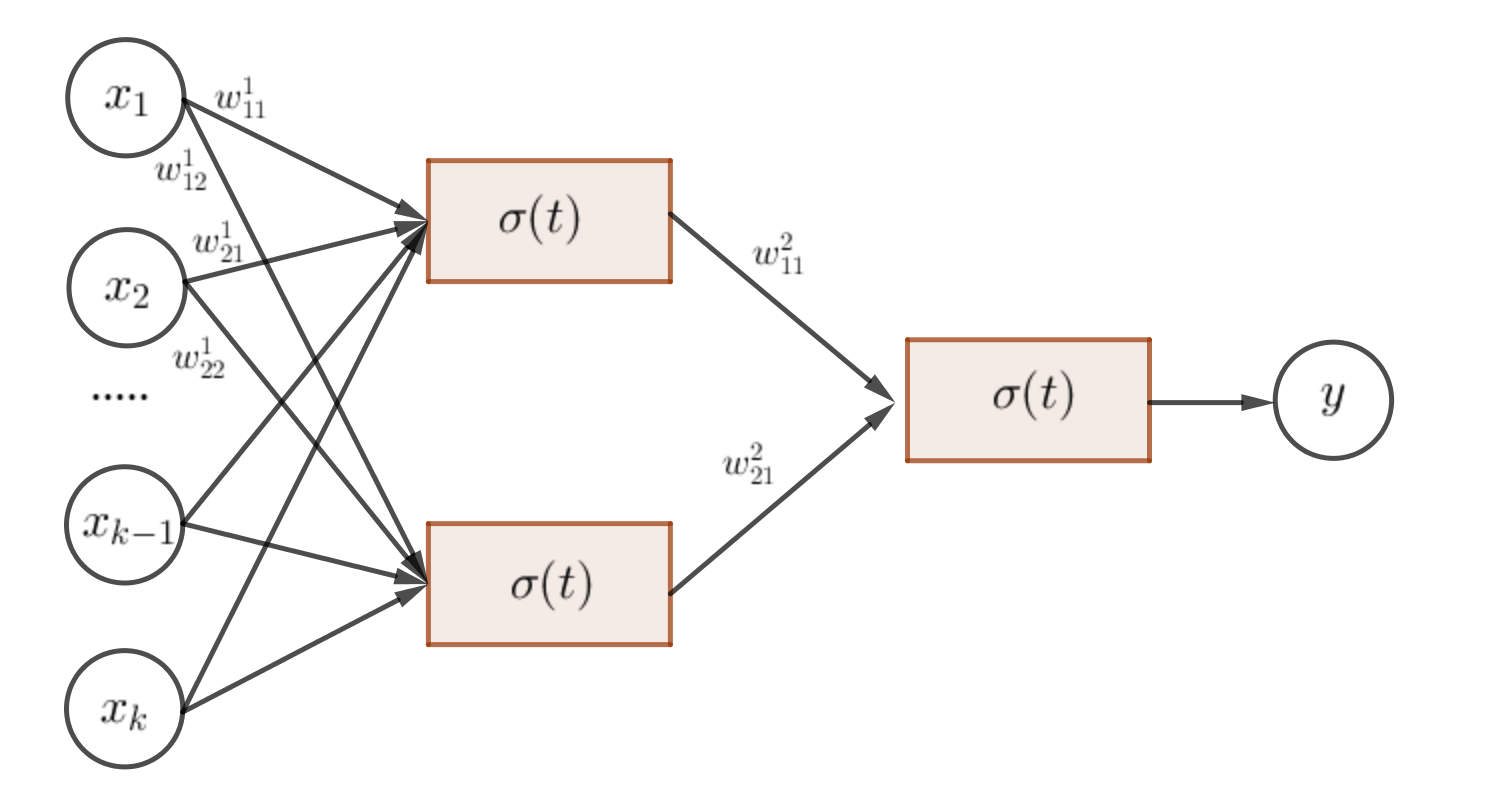
\includegraphics[width=0.7\paperwidth]{neuron_4.png}
\end{center}
\begin{equation*}
\begin{aligned}
&y = \sigma(w_{11}^2 \cdot h_1 + w_{21}^2 \cdot h_2) \\
&h_j = \sigma(\sum_i w_{ij})
\end{aligned}
\end{equation*}
\end{frame}


\begin{frame}{Две регрессии скрепили третьей}
\begin{center}
	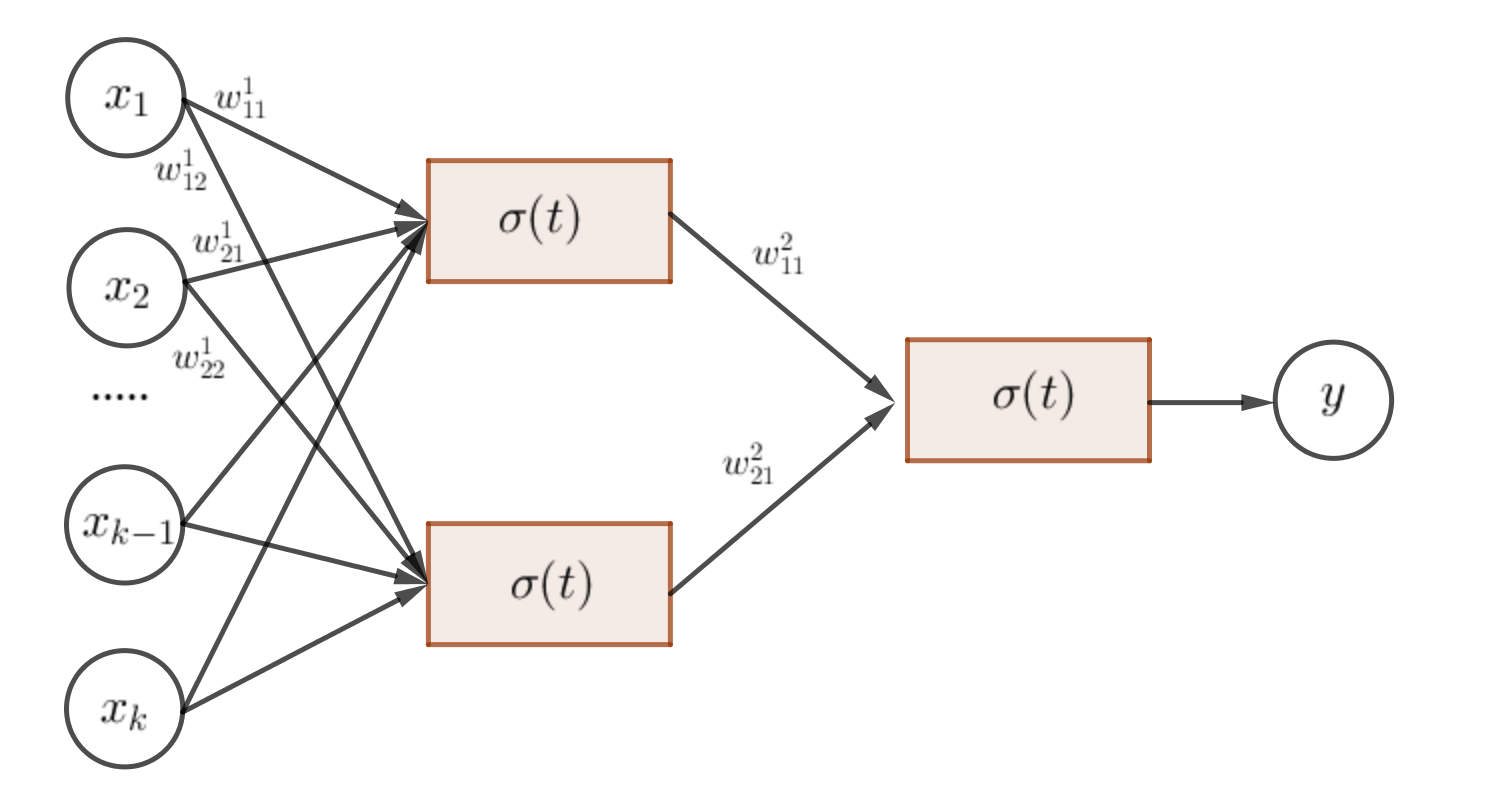
\includegraphics[width=0.7\paperwidth]{neuron_4.png}
\end{center}
\begin{equation*}
\begin{aligned}
&y = \sigma(hW) \\
&h = \sigma(XW)
\end{aligned}
\end{equation*}
\end{frame}


\begin{frame}{Армия из регрессий}
\begin{center}
	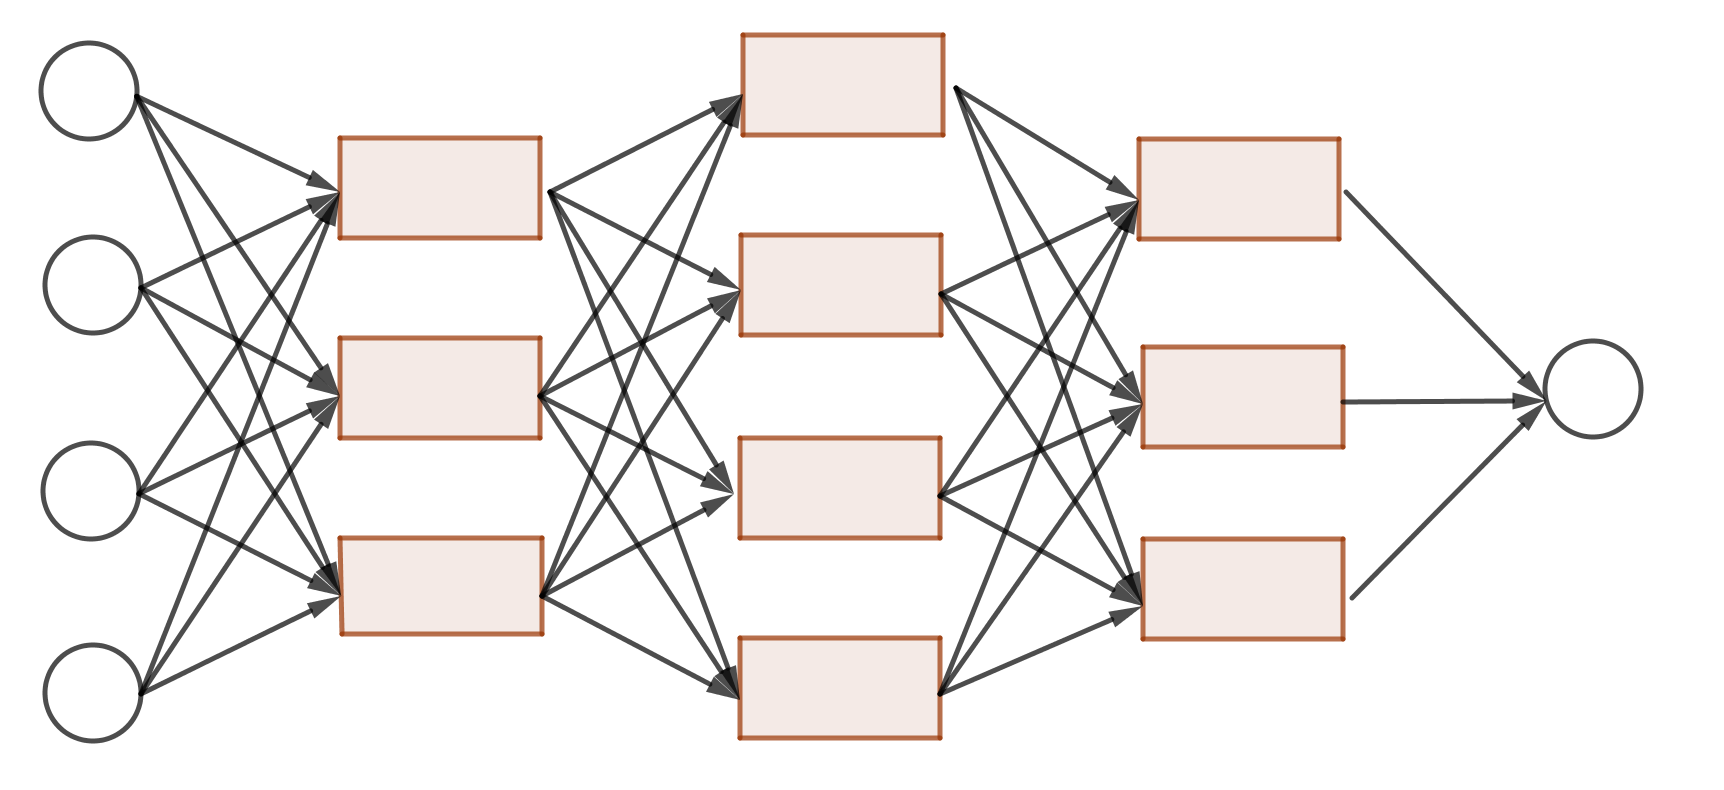
\includegraphics[width=0.8\paperwidth]{network.png}
\end{center}
\end{frame}


\begin{frame}{The Perceptron Convergence Theorem (Rosenblat, 1965)}

\begin{wideitemize}
	\item Любая непрерывная и ограниченная функция может быть сколь угодно точно аппроксимирована нейронной сетью с одним скрытым слоем с нелинейной функцией активации нейрона.
	
	\item Любая функция может быть сколь угодно точно аппроксимирована нейронной сетью с двумя скрытыми слоями с нелинейной функцией активации нейрона.
	
	\item Что ещё можно пожелать?
\end{wideitemize}
\end{frame}


{
	\usebackgroundtemplate{ 
		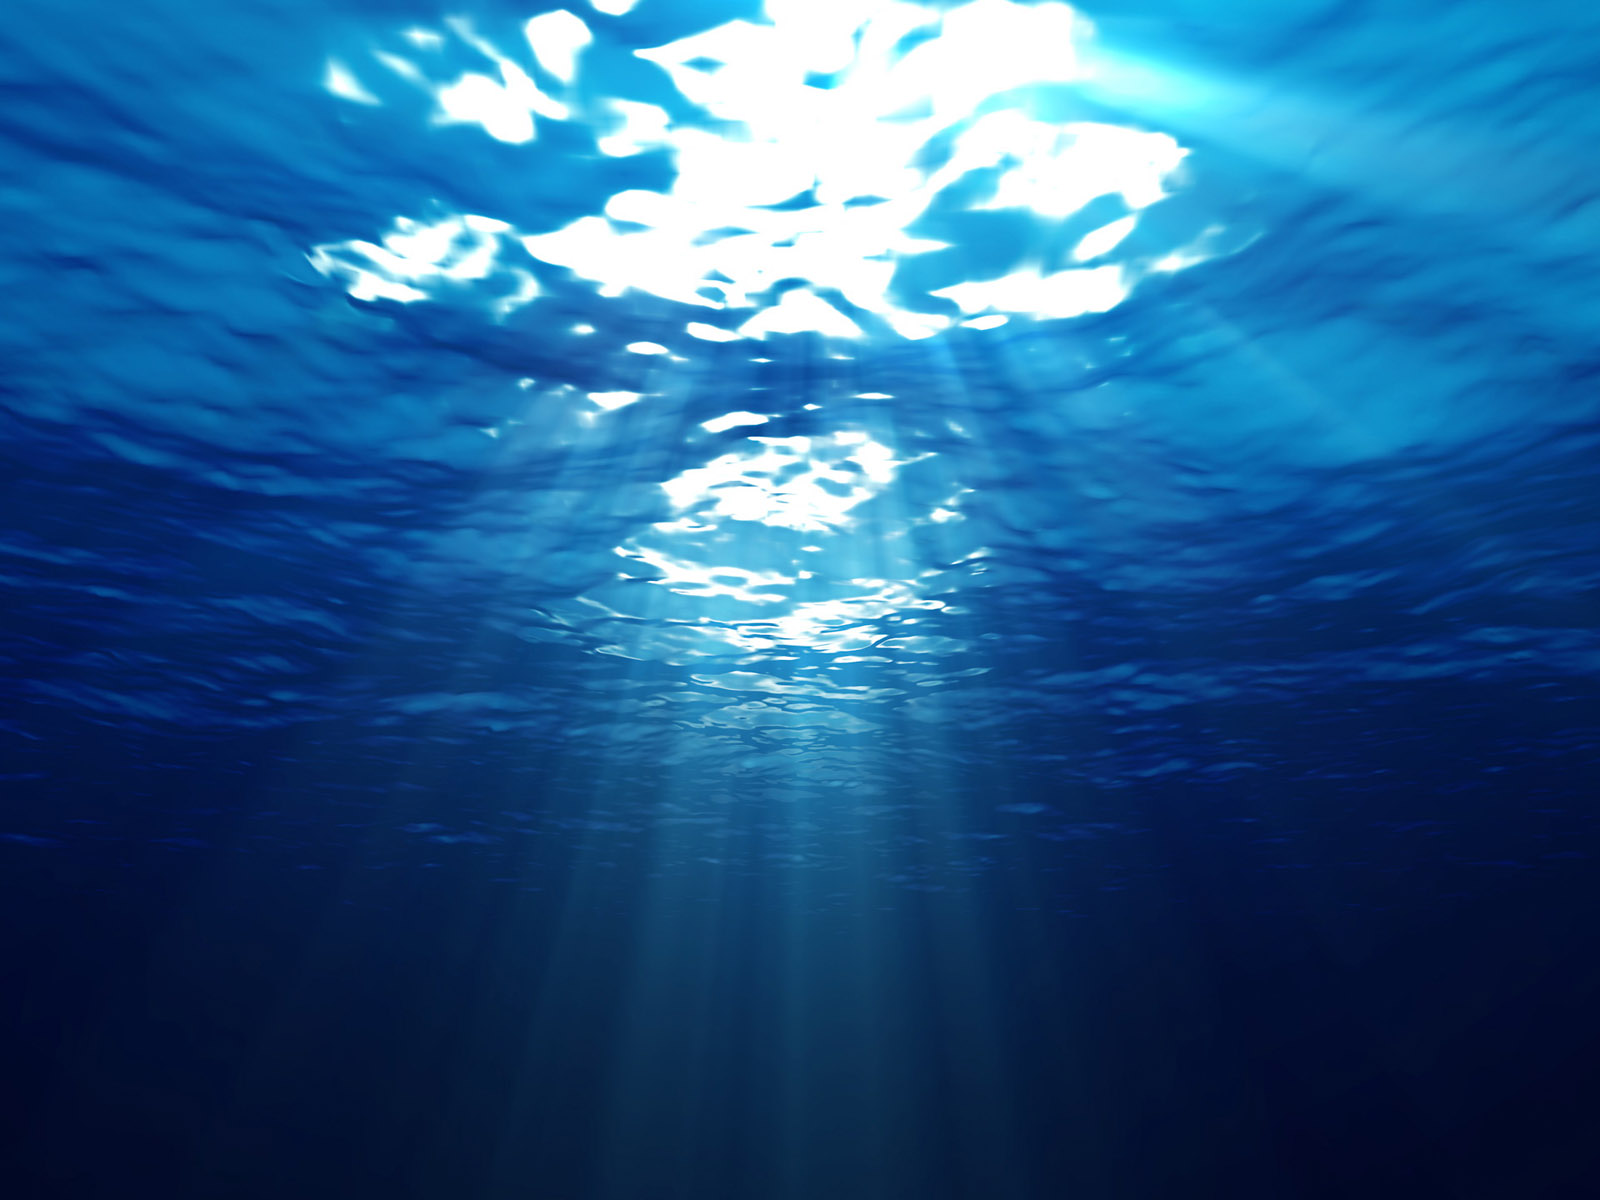
\includegraphics[width=\paperwidth]{goingdeeper.jpg}}
	\begin{frame}[fragile]
	\vspace{6.5cm}
	\begin{center}
		{\color{white} \Huge{Going Deeper}}
	\end{center}
\end{frame}
}

\begin{frame}{Мотивация}
\begin{wideitemize}
\item Перцептрон может решить любую проблему, но это дорого

\item Глубокие архитектуры часто позволяют выразить то же самое, приблизить те же функции гораздо более эффективно, чем неглубокие

\item Каждый новый слой сетки будет работать всё с более сложными фичами
\end{wideitemize}
\end{frame}


\begin{frame}{Армия из регрессий}
\begin{center}
	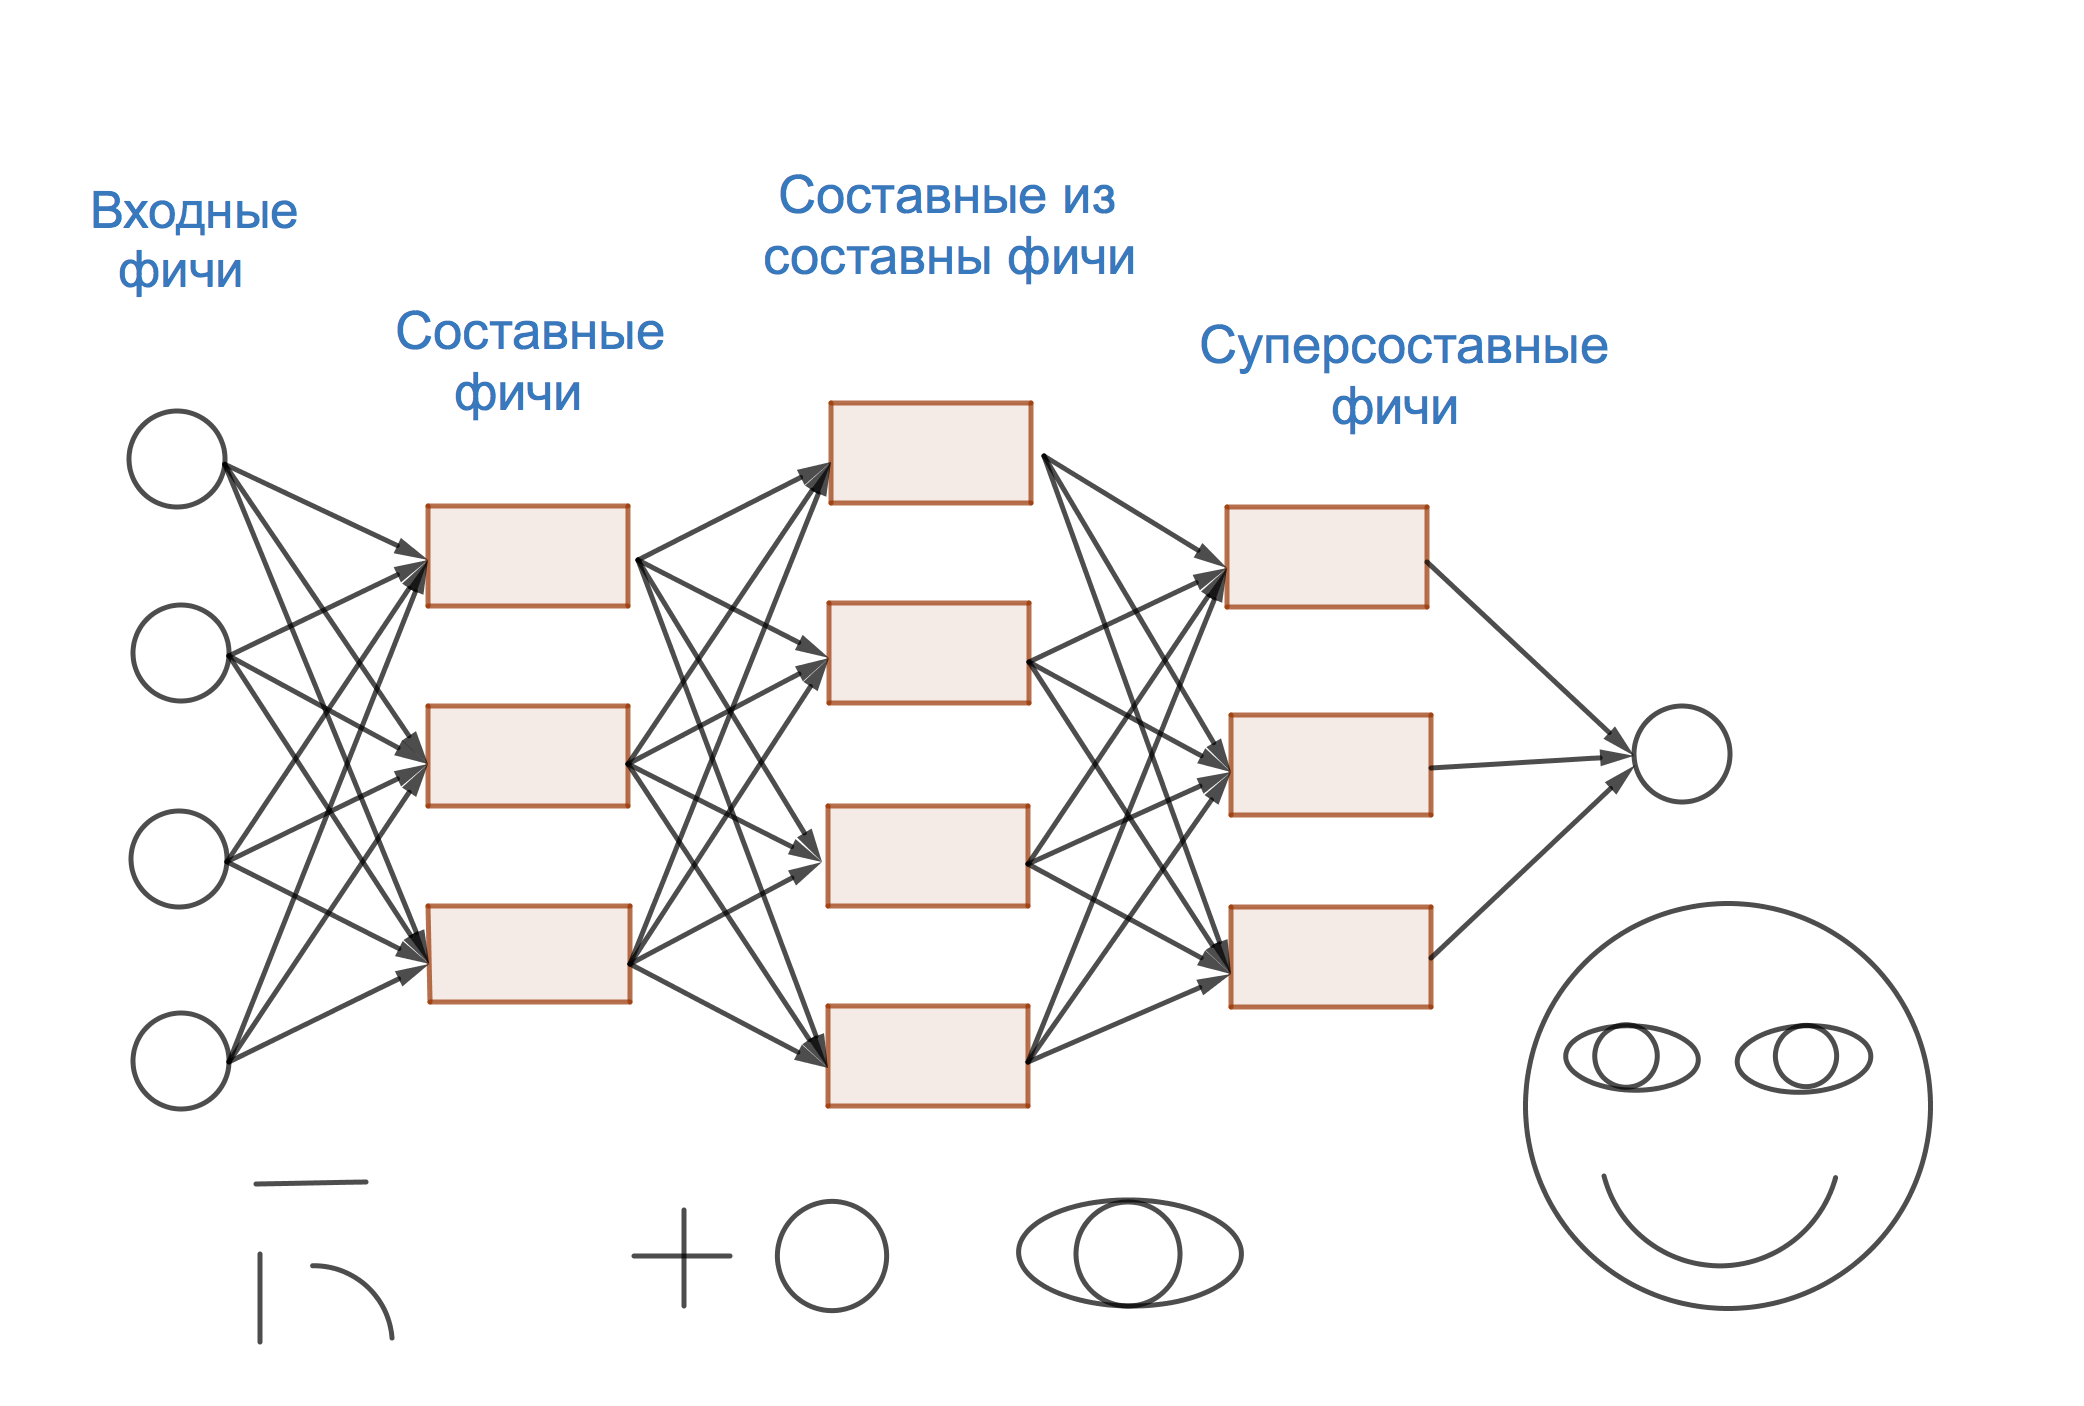
\includegraphics[width=0.73\paperwidth]{network_1.png}
\end{center}
\end{frame}


\begin{frame}{Слои бывают разными}
\begin{wideitemize}
	\item Слой, который просто взвешивает входы называется \textbf{полносвязным.}
	
	\item Слои бывают очень разными. Например, \textbf{Dropout:}  с вероятностью $p$ отключаем нейрон. Такой слой препятствует переобучению и делает нейроны более устойчивыми к случайным возмущениям.
\end{wideitemize}
\begin{center}
	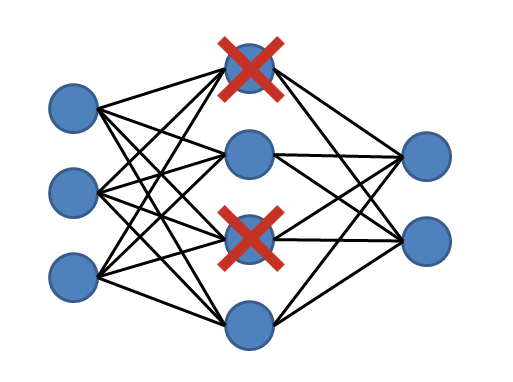
\includegraphics[width=0.3\paperwidth]{dropout.png}
\end{center}
\end{frame}


\begin{frame}{Функции активации бывают разными (сигмоид)}
\begin{center}
	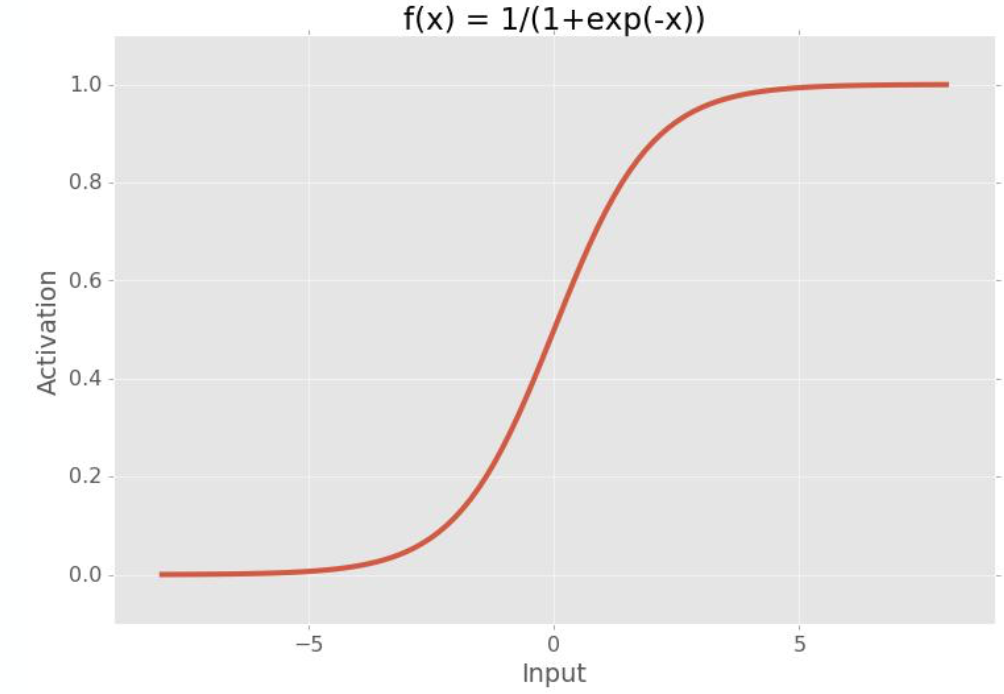
\includegraphics[width=0.65\paperwidth]{sigmoid.png}
\end{center}
\end{frame}


\begin{frame}{Линейная активация}
\begin{center}
	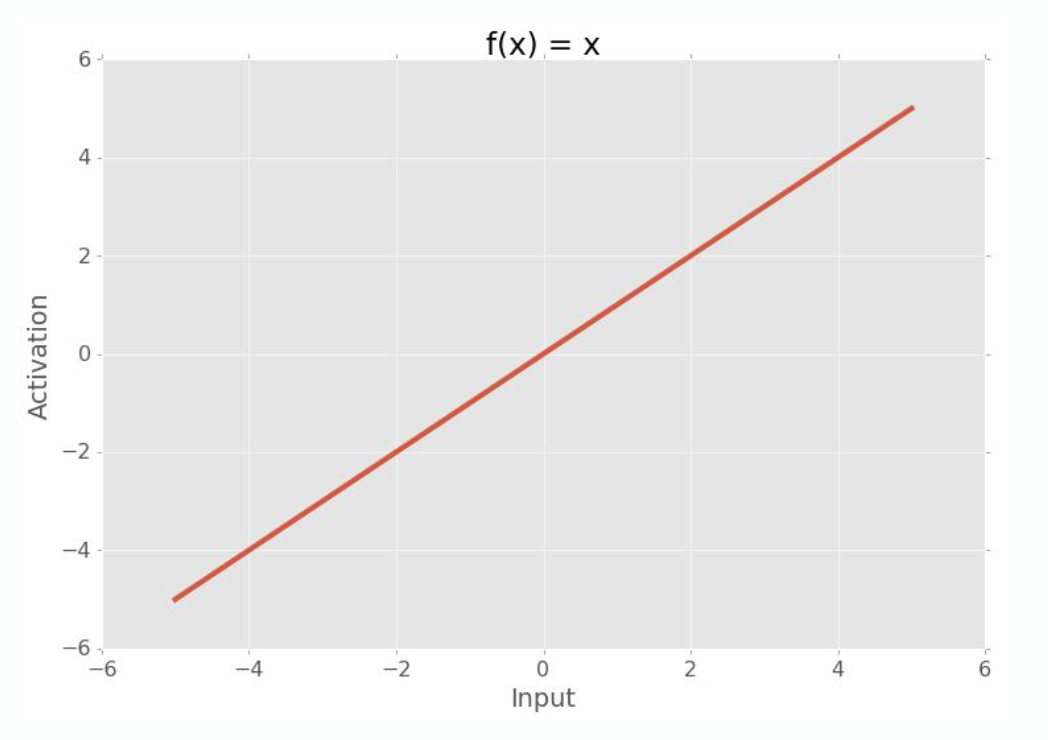
\includegraphics[width=.4\linewidth]{linear_activation.png}
\end{center}

\[ \hat y = h \cdot W_2 = X \cdot W_1 \cdot W_2 = X \cdot A \]

\begin{itemize}
	\item  После линейной активации выход снова линейный
\end{itemize}
\end{frame}


\begin{frame}{От линейной активации ... }
\begin{center}
	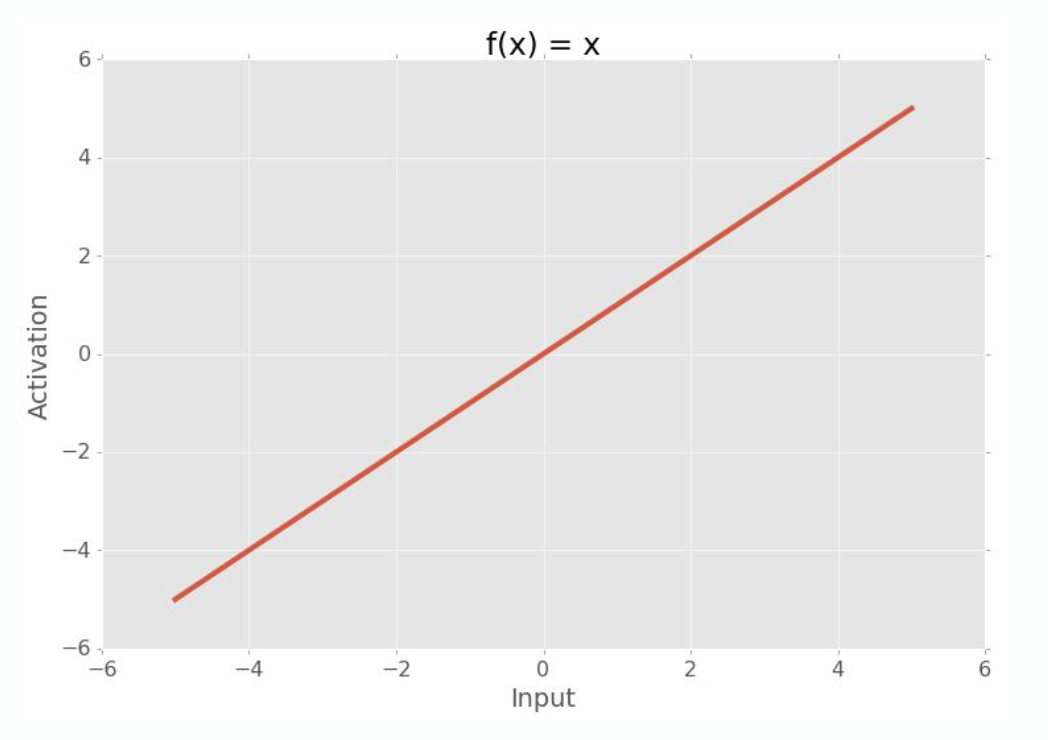
\includegraphics[width=.7\linewidth]{linear_activation.png}
\end{center}
\end{frame}


\begin{frame}{... к нелинейной (ReLU)}
\begin{center}
	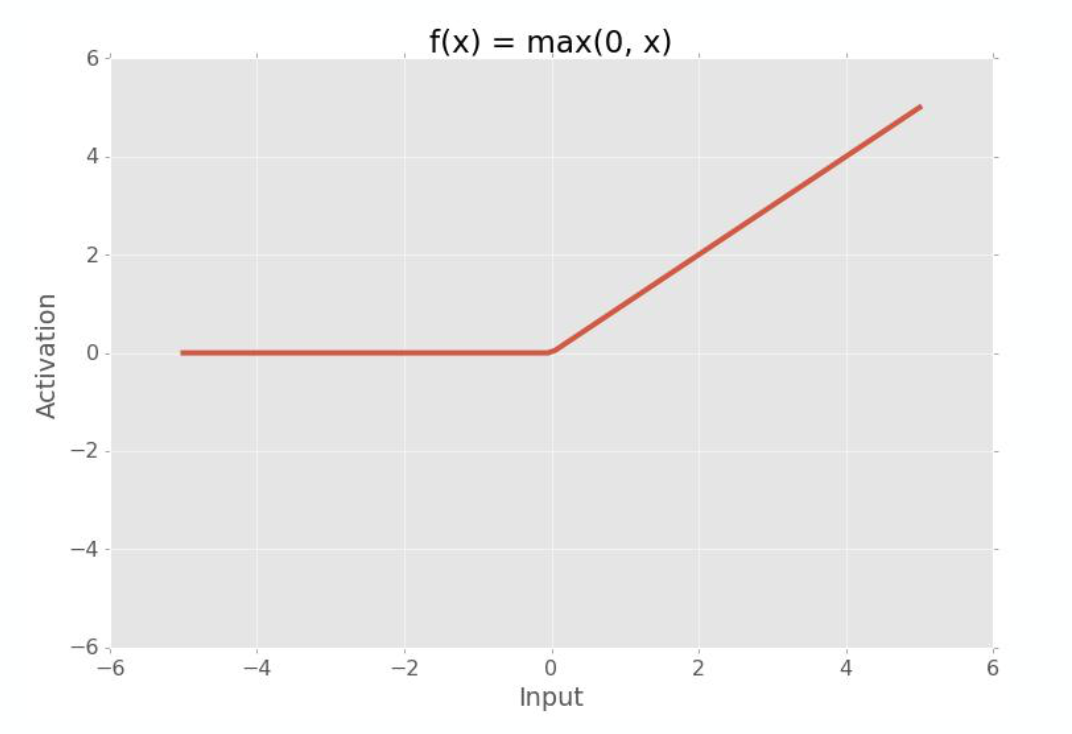
\includegraphics[width=.7\linewidth]{nonlinear_activation.png}
\end{center}
\end{frame}


\begin{frame}{Архитектуры бывают разными}
\begin{center}
	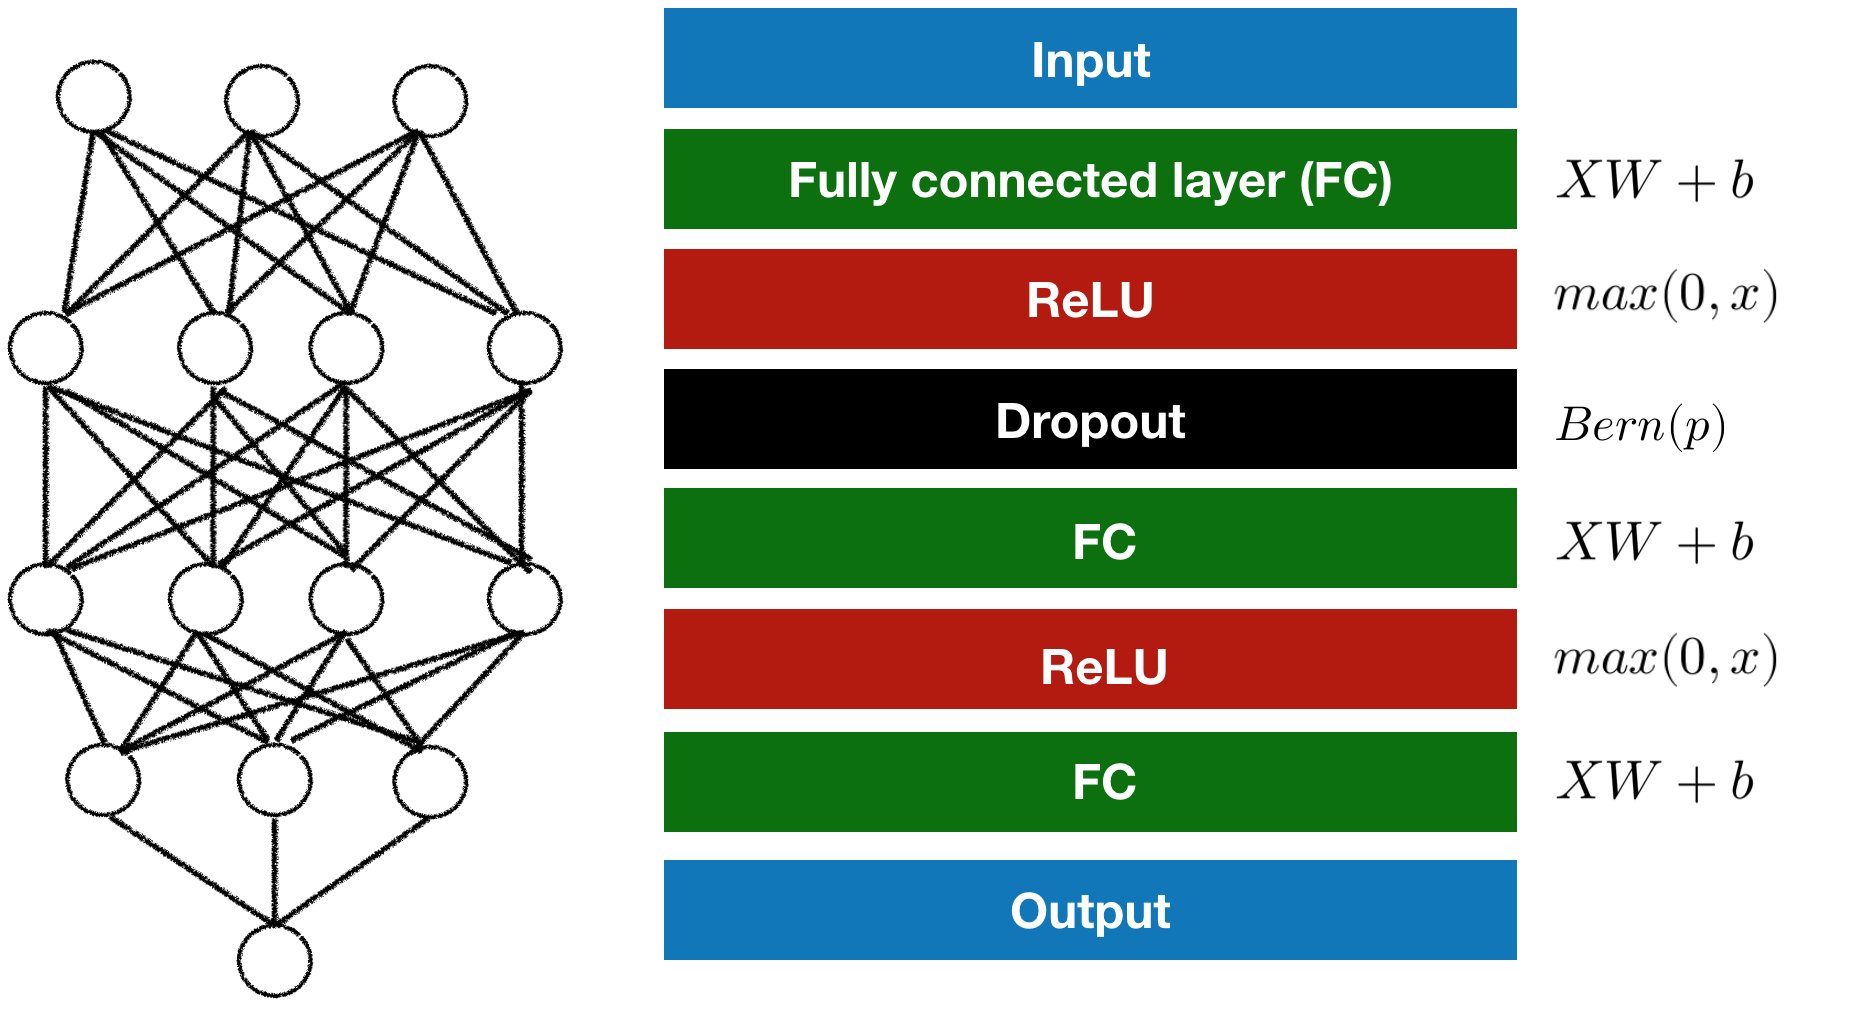
\includegraphics[width=0.75\paperwidth]{nn_lego_1.png}
\end{center}
Каждый слой — просто функция, каждая сетка — конструктор LEGO
\end{frame}


\begin{frame}{Регрессия}
\begin{center}
	\includegraphics[width=0.75\paperwidth]{nn_lego_1.png}
\end{center}
\end{frame}


\begin{frame}{Классификация}
\begin{center}
	\includegraphics[width=0.75\paperwidth]{lego_class_two.png}
\end{center}
\end{frame}


\begin{frame}{Мультиклассификация}
\begin{center}
	\includegraphics[width=0.75\paperwidth]{lego_nn_multi.png}
\end{center}
\end{frame}

\begin{frame}{Мультиклассификация}
\begin{center}
	\includegraphics[width=0.9\paperwidth]{softmax.png}
\end{center}
\end{frame}

\begin{frame}{Мультирегрессия}
\begin{center}
	\includegraphics[width=0.75\paperwidth]{nn_lego_regr.png}
\end{center}
\end{frame}

\begin{transitionframe}
	\begin{center}
		\Huge Учим нейросеть руками!
	\end{center}
\end{transitionframe}



\end{document}
